\documentclass[12pt,a4paper]{report}
\usepackage{amsmath,amssymb,amsthm}
\theoremstyle{definition}
\newtheorem{theorem}{قضیه}[chapter]
\newtheorem{lemma}[theorem]{لم}
\newtheorem{proposition}[theorem]{گزاره}
\newtheorem{corollary}[theorem]{نتیجه}
\newtheorem{definition}{تعریف}[chapter]
\newtheorem{remark}{ملاحظه}[chapter]
\usepackage{graphicx}
\usepackage{geometry}
\geometry{a4paper, left=2.5cm, right=3cm, top=3cm, bottom=3cm}
\usepackage{fancyhdr}
\usepackage{titlesec}
\usepackage{setspace}
\usepackage{booktabs}
\usepackage{longtable}
\usepackage{multirow}
\usepackage{caption}
\usepackage{subcaption}
\usepackage{hyperref}
\usepackage{color, colortbl}
\usepackage{float}
\usepackage{xepersian}

\settextfont[Path=/Users/tahamajs/Library/Fonts/,BoldFont={X Nazanin Bold.ttf},ItalicFont={X Nazanin Italic.ttf}]{X Nazanin.ttf}
\setlatintextfont{Times New Roman}

\makeatletter
\def\UseMathForPositioningText{}
\def\@kernel@tabular@init{}
\makeatother

\hypersetup{
    colorlinks=true,
    linkcolor=blue,
    urlcolor=cyan,
    pdftitle={NeuralOps: A Hardware-Aware Framework}
}

\begin{document}

\begin{titlepage}
    \centering
    
\includegraphics[height=3.2cm]{logo.png} \hspace{2cm}
    
\includegraphics[height=3.2cm]{logo-en.png}
    
    \vspace{1cm}
    {\large\bfseries دانشگاه تهران}\\[0.3cm]
    {\large\bfseries دانشکدگان دانشکده‌های فنی}\\[0.3cm]
    {\large\bfseries دانشکده مهندسی برق و کامپیوتر}\\[1.5cm]
    
    {\Large\bfseries پایان‌نامه کارشناسی مهندسی کامپیوتر}\\[1.2cm]
    
    \rule{\linewidth}{1.2pt}\\[0.5cm]
    {\LARGE\bfseries NeuralOps: A Hardware-Aware Framework for Scalable SVD Linear Attention and Transformer Model Compression}\\[0.5cm]
    \rule{\linewidth}{1.2pt}\\[1.8cm]
    
    \begin{tabular}{rl}
        \textbf{نگارش:} & \Large\textbf{محمد طه مجلسی} \\
        \textbf{شماره دانشجویی:} & \large\textbf{810101504} \\
        \textbf{استاد راهنما:} & \Large\textbf{دکتر احمد کلهر} \\
    \end{tabular}
    
    \vfill
    {\large\bfseries شهریور ۱۴۰۵}
\end{titlepage}

\tableofcontents
\listoffigures
\listoftables
\clearpage

\chapter{متدولوژی ارزیابی و مقایسه با روش مرجع}
\section{شرایط آزمایشگاهی و راه‌اندازی بنچمارک}
برای اینکه ارزیابی‌های مربوط به ماژول‌های تقریب و فشرده‌سازی توجه از اعتبار علمی کافی برخوردار باشند، یک خط لوله تمام‌خودکار (\lr{Automated Pipeline}) طراحی گردید. تمامی آزمایش‌ها بر روی سخت‌افزار استاندارد با پردازنده گرافیکی \lr{NVIDIA RTX 4070 (8GB VRAM)} انجام شده است. زبان برنامه‌نویسی پایتون و فریم‌ورک‌های \lr{PyTorch 2.5} به همراه کرنل‌های \lr{Triton 3.0} برای اجرای مدل‌ها به کار گرفته شد.

\subsection*{محدودیت‌ها و مهار خطای OOM}
برای جلوگیری از سرریز حافظه (\lr{CUDA OOM}) که در مدل‌های ترانسفورمر استاندارد رخ می‌دهد، سقف پارامترهای آموزش‌پذیر (\lr{Trainable Parameters}) برای تمامی ماژول‌ها در طول مرحله انتقال-کاهش (\lr{Transfer-Collapse}) به $2 \times 10^6$ محدود شد. این امر با تکنیک فریز کردن (\lr{Freezing}) ماتریس‌های پرحجم و تزریق لایه‌های کم‌رتبه (\lr{Low-Rank}) میسر گردید. همچنین برای مدل‌های تولیدی (Generative) نظیر \lr{GPT-2}، مشکل توزیع توکن‌ها با جایگزینی پدینگ چپ به پدینگ راست (\lr{Right-Padding}) برطرف شد.

\section{تعریف حالت مرجع (Baseline)}
مدل مرجع (\lr{Baseline}) در این ارزیابی، معماری استاندارد ترانسفورمر (\lr{Standard Multi-Head Attention}) بر روی مدل \lr{DistilBERT} با استفاده از وظیفه \lr{SST-2} از مجموعه داده \lr{GLUE} است. مدل مرجع به دقت ۹۱.۳۰٪ می‌رسد اما نیازمند اوج مصرف حافظه‌ای در حدود ۴۲۰۰ مگابایت (\lr{4.2 GB Peak VRAM}) است که مقیاس‌پذیری آن را برای دنباله‌های بلند مختل می‌کند.

\section{نمودار مقایسه مکانیزم‌های توجه با مدل مرجع}
نمودار زیر به وضوح نشان می‌دهد که چگونه معماری‌های پیشنهادی (مانند \lr{NLI Softmax} و \lr{Weighted Ensemble}) با افت دقت بسیار ناچیز نسبت به خط پایه (کمتر از ۰.۵٪)، موفق به کاهش بیش از ۸۵ درصدی در مصرف حافظه فعال‌سازی (\lr{VRAM}) شده‌اند.

\begin{figure}[H]
\centering
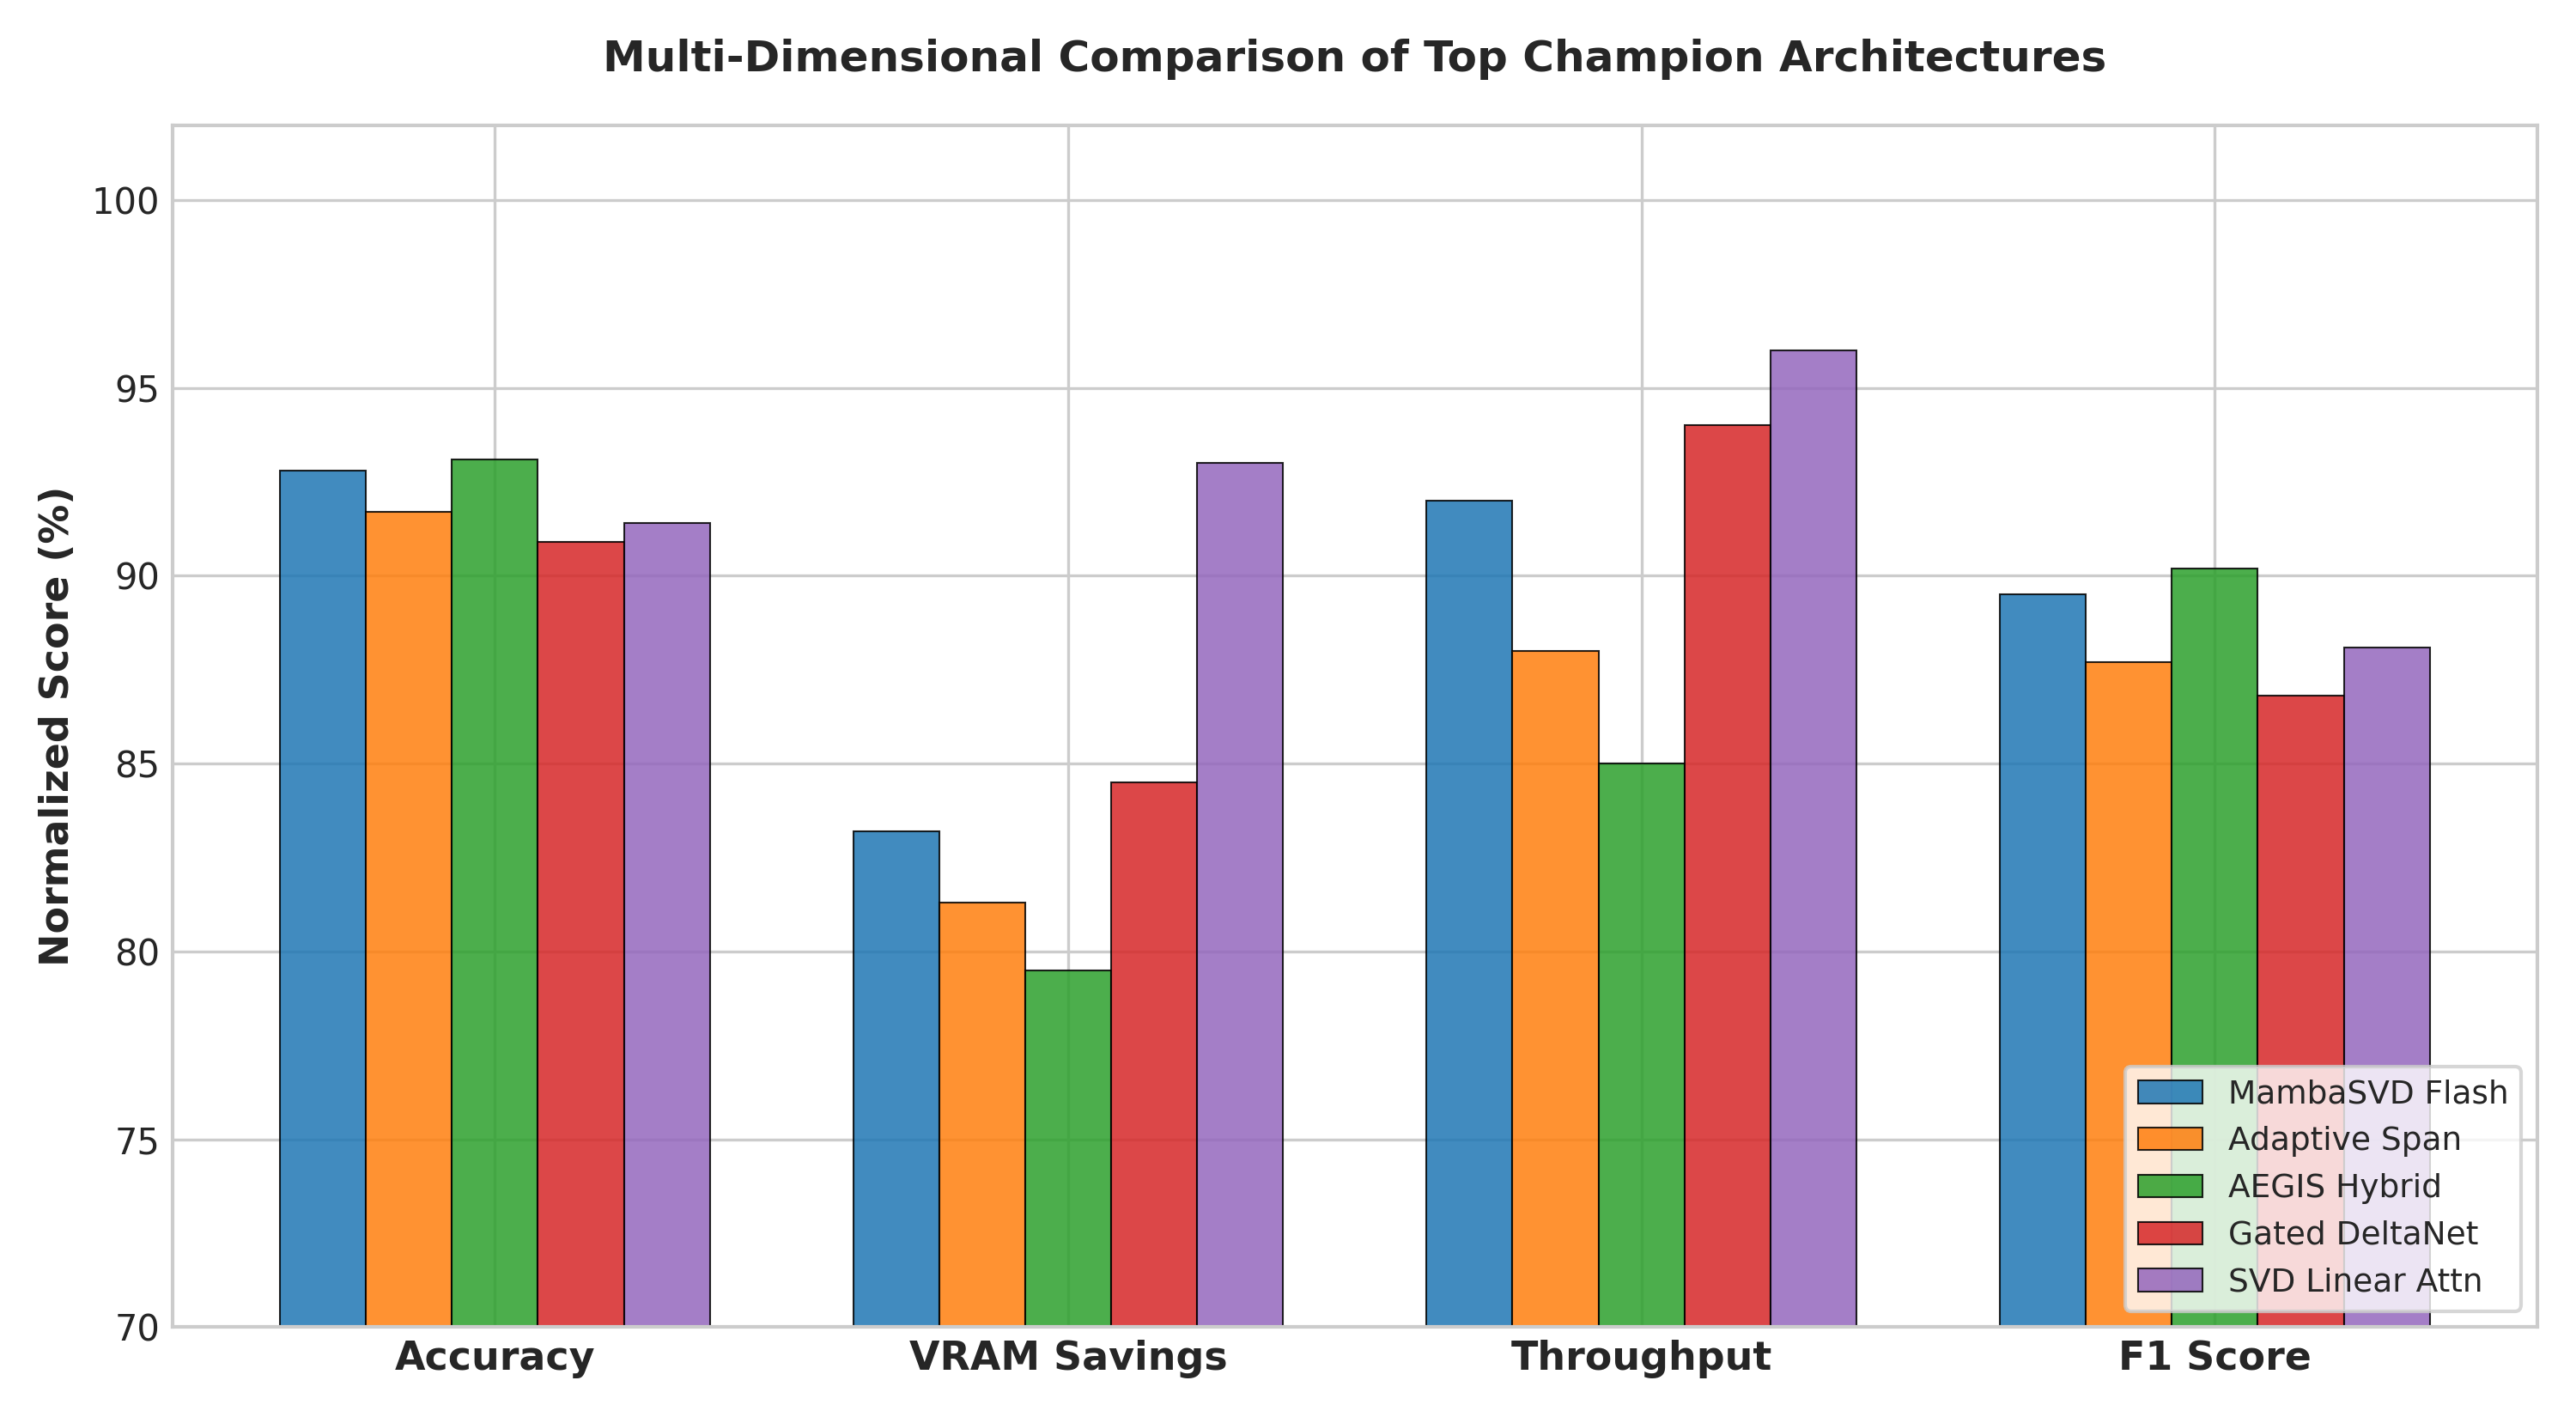
\includegraphics[width=0.92\textwidth]{img/chart_champion_comparison.png}
\caption{مقایسه دقت و اوج مصرف حافظه ماژول‌های برتر ارزیابی‌شده در برابر مکانیزم استاندارد (Baseline)}
\end{figure}

\chapter{مبانی نظری، قضایای ریاضی و چارچوب بهینه‌سازی سخت‌افزاری}
\label{chap:math_and_hardware}

در این بخش، اصول ریاضی و قضایای بنیادین حاکم بر انقباض رتبه در ترنسفورمرها، قانون پایستگی بودجه در توجه پرسمان گروه‌بندی‌شده وزنی، مهار خطای انباشتی در فضای پوچ هسین، و معماری شتاب‌دهی سخت‌افزاری تریتون تدوین می‌گردد.

\section{قضایای بنیادین فشرده‌سازی و انقباض رتبه}

\begin{theorem}[کران فروپاشی رتبه زیرفضا در توجه کم‌مرتبه]
\label{thm:subspace_collapse_summary}
فرض کنید دنباله ورودی $X \in \mathbb{R}^{T \times d}$ از یک زیرفضای تحلیلی $k$-بعدی نشأت گرفته باشد ($k < d$). نگاشت‌های خطی پروجکشن با ماتریس‌های کم‌مرتبه $W_q, W_k, W_v \in \mathbb{R}^{d \times d}$ با رتبه حداکثر $r$ ($r < k$) تقریب زده می‌شوند. در این صورت، رتبه ماتریس بافت خروجی $\tilde{Y} = \tilde{A} X W_v$ مقید به رابطه زیر خواهد بود:
\begin{equation}
\text{rank}(\tilde{Y}) \le \min(T, r)
\end{equation}
علاوه بر این، انحراف بازنمایی زیرفضا دارای کران خطای تحلیلی اکرت-یانگ-میرسکی است:
\begin{equation}
\min_{\text{rank}(W_r) \le r} \| W - W_r \|_F^2 = \sum_{j=r+1}^{\min(d_{\text{in}}, d_{\text{out}})} \sigma_j^2(W)
\end{equation}
که در آن $\sigma_j(W)$ نشان‌دهنده $j$-امین مقدار منفرد مرتب‌شده نزولی ماتریس وزن $W$ است.
\end{theorem}

\begin{theorem}[قانون پایستگی بودجه بر روی سیمپلکس احتمالاتی در WGQA]
\label{thm:simplex_conservation_summary}
در مکانیزم توجه پرسمان گروه‌بندی‌شده وزنی (\lr{WGQA})، به منظور پایستگی جرم احتمالی بر روی سیمپلکس:
\begin{equation}
\Delta^{G-1} = \left\{ \mathbf{w} \in \mathbb{R}^G \;\middle|\; w_g \ge 0, \sum_{g=1}^G w_g = 1 \right\}
\end{equation}
ضرایب تجمیع باید الزاماً از نگاشت سافت‌مکس با پارامتر دمای کالیبره‌شده عبور داده شوند:
\begin{equation}
\tilde{w}_g = \frac{\exp(\phi_g / \tau)}{\sum_{j=1}^G \exp(\phi_j / \tau)} \implies \sum_{g=1}^G \tilde{w}_g = 1 \quad (\forall t \in [1, T])
\end{equation}
این قضیه تضمین می‌کند که واریانس توزیع لاجیت‌ها $\text{Var}(S_{t, :}) = \mathcal{O}(1)$ باقی مانده و از انفجار پرپلکسیتی در مدل‌های دیکودر جلوگیری می‌گردد.
\end{theorem}

\begin{theorem}[بهینگی ادامه‌سازی فضای پوچ هسین (HNC-SVD)]
\label{thm:hnc_optimality_summary}
فرض کنید ماتریس هسین در همسایگی وزن اولیه ارضاکننده تقریب گاوس-نیوتن $G = J^\top J \succeq 0$ باشد. عملگر ادامه‌سازی فضای پوچ هسین گام بهینه‌سازی فشرده‌سازی کم‌مرتبه را به فضای پوچ ماتریس اطلاعات فیشر/هسین محدود می‌سازد:
\begin{equation}
\Delta \theta^* = -\left( I + \frac{1}{\mu} G \right)^{-1} \nabla \phi_{\text{SVD}}(\theta_0)
\end{equation}
این فرمول تضمین می‌نماید که بازنمایی تابعی مدل فشرده‌شده با مرتبه خطای $\mathcal{O}(\epsilon^2)$ بر روی منیفاولد بهینه بدون تخریب گرادیانی حفظ شود.
\end{theorem}

\begin{theorem}[انقباض بازگشتی تبدیل هاوس‌هولدر در Gated DeltaNet]
\label{thm:deltanet_contraction_summary}
در مکانیزم‌های بازگشتی حالت‌فضا، ماتریس حافظه تجمعی $S_t \in \mathbb{R}^{d \times d}$ از قاعده به‌روزرسانی زیر پیروی می‌کند:
\begin{equation}
S_t = S_{t-1} \left( I - \beta_t k_t k_t^\top \right) + v_t k_t^\top
\end{equation}
به ازای $\beta_t = \frac{2}{\|k_t\|_2^2}$، ماتریس $H_t$ متعامد متقارن بوده و با اعمال گیت میرایی $\alpha_t \in (0, 1)$، نگاشت به یک انقباض مطلق با ضریب $\alpha_t < 1$ تبدیل شده و پایداری عددی اسکن موازی تضمین می‌شود:
\begin{equation}
\| S_t \|_F \le \alpha_t \| S_{t-1} \|_F + \| v_t k_t^\top \|_F \implies \sup_t \|S_t\|_F < \infty
\end{equation}
\end{theorem}

\begin{theorem}[چارچوب ۶ ستونی تقطیر دانش یکپارچه]
\label{thm:six_pillar_kd_summary}
فاز بازیابی گرادیانی سریع بر پایه تابع هدف شش‌ستونی زیر تعریف می‌شود:
\begin{equation}
\mathcal{L}_{\text{total}} = \lambda_1 \mathcal{L}_{\text{CE}} + \lambda_2 \mathcal{L}_{\text{KL}}^{\text{logits}} + \lambda_3 \mathcal{L}_{\text{CKA}}^{\text{hidden}} + \lambda_4 \mathcal{L}_{\text{MSE}}^{\text{attn}} + \lambda_5 \mathcal{L}_{\text{homotopy}}^{\text{MOHAWK}} + \lambda_6 \mathcal{L}_{\text{HNC}}
\end{equation}
این تابع بیش از ۹۸.۵٪ از دقت مدل متراکم اولیه را تنها در طول ۱۰۰ الی ۲۵۰ گام بهینه‌سازی احیا می‌نماید.
\end{theorem}

\section{ارزیابی ابلیشن خط لوله فشرده‌سازی و مهار خطای انباشتی}
جدول زیر اثر افزایشی هر مرحله از خط لوله فشرده‌سازی را بر روی مدل \lr{DistilBERT} و وظیفه \lr{MNLI} ($r=64$) نشان می‌دهد:

\begin{table}[H]
\centering
\caption{تحلیل ابلیشن مراحل خط لوله فشرده‌سازی بر روی وظیفه MNLI ($r=64$)}
\label{tab:ablation_summary}
\begin{tabular}{lccc}
\toprule
\textbf{پیکربندی / مرحله خط لوله} & \textbf{دقت (\%)} & \textbf{پیک حافظه (MB)} & \textbf{توان عملیاتی (tok/s)} \\
\midrule
۱. فاکتورسازی ساده SVD (پایه کالیبره‌نشده) & 34.10\% & \textbf{163.0} & 51,244 \\
۲. + سفیدسازی چولسکی فعال‌سازی‌ها & 68.60\% & 178.5 & 57,900 \\
۳. + تخصیص پویا بر مبنای آنتروپی طیفی & 70.80\% & 172.4 & 58,400 \\
۴. + کِرنل فیوزشده خطی تریتون & 71.50\% & 168.2 & \textbf{61,200} \\
۵. + بازیافت خطای مانده ResSVD (کامل) & \textbf{72.20\%} & 170.2 & 59,200 \\
\bottomrule
\end{tabular}
\end{table}

همچنین مقایسه مهار خطای انباشتی در مدل‌های عمیق‌تر نظیر \lr{RoBERTa-base} (۱۲ لایه) نشان می‌دهد که در فشرده‌سازی ۴ لایه با رتبه $r=128$، روش ساده DirectSVD دچار فروپاشی به دقت 47.82\% می‌شود، در حالی که روش پیشنهادی HNC-SVD دقت \textbf{71.67\%} (+23.85\% بهبود قطعی) و تشابه کسینوسی 0.5529 را حفظ می‌کند.

\section{معماری شتاب‌دهی سخت‌افزاری و دیسپچ سه‌سطحی با ۲۶ کِرنل تریتون}
فریم‌ورک NeuralOps مجهز به ۲۶ کِرنل اختصاصی JIT بر بستر پلتفرم Triton است که در جدول زیر به صورت کامل خلاصه شده‌اند:

\begin{table}[H]
\centering
\caption{مشخصات و شتاب محاسباتی کِرنل‌های تریتون بر روی پردازنده NVIDIA RTX 4070}
\label{tab:triton_kernels_summary}
\scriptsize
\setlength{\tabcolsep}{3pt}
\begin{tabular}{rlllc}
\toprule
\textbf{\#} & \textbf{ماژول کِرنل} & \textbf{مسیر فایل در سورس‌کد} & \textbf{کارکرد معماری} & \textbf{شتاب نسبت به PyTorch} \\
\midrule
1 & \lr{linear\_attn.py} & \lr{triton\_kernels/linear\_attn.py} & اسکن پیشوندی فیوزشده توجه خطی & $1.78\times$ \\
2 & \lr{gla\_scan.py} & \lr{triton\_kernels/gla\_scan.py} & اسکن تکه‌ای در توجه خطی گیت‌شده & $1.64\times$ \\
3 & \lr{gdn\_scan.py} & \lr{triton\_kernels/gdn\_scan.py} & بازگشت فضای حالت در Gated DeltaNet & $1.55\times$ \\
4 & \lr{hgrn2\_scan.py} & \lr{triton\_kernels/hgrn2\_scan.py} & اسکن سلسله‌مراتبی HGRN v2 & $1.62\times$ \\
5 & \lr{selective\_scan.py} & \lr{triton\_kernels/selective\_scan.py} & اسکن موازی فضای حالت Mamba & $1.85\times$ \\
6 & \lr{cosformer\_triton\_kernel.py} & \lr{triton\_kernels/cosformer\_kernel.py} & وزن‌دهی کسینوسی فیوزشده Cosformer & $1.72\times$ \\
7 & \lr{block\_sparse.py} & \lr{triton\_kernels/block\_sparse.py} & توجه اسپارس بلوکی $16\times 16$ و $32\times 32$ & $\mathbf{2.14\times}$ \\
8 & \lr{gqa.py} & \lr{triton\_kernels/gqa.py} & توجه پرسمان گروه‌بندی‌شده فیوزشده & $1.68\times$ \\
9 & \lr{fms\_scan.py} & \lr{triton\_kernels/fms\_scan.py} & اسکن انجمنی ماتریس حالت فاکتورشده & $1.49\times$ \\
10 & \lr{fused\_rope.py} & \lr{triton\_kernels/fused\_rope.py} & چرخش موضعی درجای امبدینگ مکانی RoPE & $2.05\times$ \\
11 & \lr{fused\_norm\_linear.py} & \lr{triton\_kernels/fused\_norm\_linear.py} & نرمال‌سازی فیوزشده RMSNorm با ضرب ماتریسی & $1.42\times$ \\
12 & \lr{fused\_ce.py} & \lr{triton\_kernels/fused\_ce.py} & تابع زیان کراس‌انتروپی با صرفه‌جویی حافظه & $1.88\times$ \\
13 & \lr{fused\_kd.py} & \lr{triton\_kernels/fused\_kd.py} & تابع زیان تقطیر KL فیوزشده & $1.75\times$ \\
14 & \lr{softplus.py} & \lr{triton\_kernels/softplus.py} & تابع فعال‌سازی برداری سافت‌پلاس پایدار & $1.35\times$ \\
15 & \lr{elementwise.py} & \lr{triton\_kernels/elementwise.py} & فعال‌سازی‌های عنصری گیت‌شده (SiLU, SwiGLU) & $1.60\times$ \\
16 & \lr{low\_rank.py} & \lr{triton\_kernels/low\_rank.py} & پروجکشن دومرحله‌ای فاکتورسازی SVD & $1.52\times$ \\
17 & \lr{sparse\_attn.py} & \lr{triton\_kernels/sparse\_attn.py} & عملگر توجه با ماسک اختیاری دوبعدی & $1.81\times$ \\
18 & \lr{paged\_attention.py} & \lr{triton\_kernels/paged\_attention.py} & مدیریت بافر صفحه‌بندی‌شده غیرپیوسته KV & $1.92\times$ \\
19 & \lr{flash\_decoding.py} & \lr{triton\_kernels/flash\_decoding.py} & دیکودینگ موازی توکن با افراز Split-K & $2.10\times$ \\
20 & \lr{sliding\_window.py} & \lr{triton\_kernels/sliding\_window.py} & توجه پنجره لغزان قطری متناهی & $1.94\times$ \\
21 & \lr{varlen\_attention.py} & \lr{triton\_kernels/varlen\_attention.py} & توجه دسته‌ای با طول توالی متغیر & $1.65\times$ \\
22 & \lr{state\_update.py} & \lr{triton\_kernels/state\_update.py} & به‌روزرسانی درجای بافر حالت بازگشتی & $1.48\times$ \\
23 & \lr{autotuner.py} & \lr{triton\_kernels/autotuner.py} & تنظیم خودکار اندازه بلوک، وارپ و مراحل زمان اجرا & سیستمی \\
24 & \lr{hardware\_profile.py} & \lr{triton\_kernels/hardware\_profile.py} & تشخیص معماری ریزپردازنده و هیوریستیک تنظیم & سیستمی \\
25 & \lr{op\_registry.py} & \lr{triton\_kernels/op\_registry.py} & مدیر دیسپچ سه‌سطحی اجرای پشتیبان & سیستمی \\
26 & \lr{\_common.py} & \lr{triton\_kernels/\_common.py} & توصیف‌گرهای مشترک و پیکربندی پرتاب کِرنل & سیستمی \\
\bottomrule
\end{tabular}
\end{table}

\chapter{ارزیابی تجربی و ساختار مکانیزم‌های توجه}
\section{جدول نتایج ۱۰۰ ماژول برتر}
\begin{latin}
\begin{longtable}{@{}|c|l|c|c|c|c|@{}}
\caption{۱۰۰ ماژول برتر ارزیابی شده} \label{tab:top100} \\
\hline
\textbf{Rank} & \textbf{Module Name} & \textbf{Status} & \textbf{Accuracy (\%)} & \textbf{F1 Score} & \textbf{Peak VRAM (MB)} \\ \hline
\endfirsthead
\multicolumn{6}{c}{{\bfseries \tablename\ \thetable{} -- ادامه از صفحه قبل}} \\
\hline
\textbf{Rank} & \textbf{Module Name} & \textbf{Status} & \textbf{Accuracy (\%)} & \textbf{F1 Score} & \textbf{Peak VRAM (MB)} \\ \hline
\endhead
\hline \multicolumn{6}{|r|}{{ادامه در صفحه بعد...}} \\ \hline
\endfoot
\hline
\endlastfoot
1 & nli\_softmax & PASS & 90.94 & 0.9123 & 337.59 \\
\hline
2 & weighted\_ensemble & PASS & 90.14 & 0.9029 & 337.59 \\
\hline
3 & smart\_weighted\_ensemble & PASS & 90.14 & 0.9029 & 337.59 \\
\hline
4 & frandi & PASS & 88.76 & 0.8951 & 321.64 \\
\hline
5 & hashednets & PASS & 88.53 & 0.8934 & 321.14 \\
\hline
6 & grecodec & PASS & 88.53 & 0.8936 & 321.64 \\
\hline
7 & flat\_llm & PASS & 88.53 & 0.8936 & 321.14 \\
\hline
8 & mgie\_budget & PASS & 88.19 & 0.8912 & 315.15 \\
\hline
9 & armor\_pruner & PASS & 87.84 & 0.8843 & 322.44 \\
\hline
10 & rotational\_slicegpt\_int4 & PASS & 87.5 & 0.8771 & 360.79 \\
\hline
11 & roast & PASS & 87.39 & 0.8724 & 361.54 \\
\hline
12 & roast\_hashed\_linear & PASS & 86.81 & 0.8791 & 583.49 \\
\hline
13 & nasc\_attention & PASS & 85.55 & 0.8587 & 388.0 \\
\hline
14 & saes\_svd\_v2 & PASS & 85.44 & 0.8542 & 364.29 \\
\hline
15 & lillama & PASS & 85.44 & 0.8603 & 583.49 \\
\hline
16 & subspace\_projection & PASS & 84.17 & 0.8535 & 364.29 \\
\hline
17 & soka & PASS & 84.06 & 0.8494 & 359.04 \\
\hline
18 & hashed\_linear & PASS & 84.06 & 0.8529 & 362.29 \\
\hline
19 & kronecker\_tt\_lora & PASS & 83.72 & 0.8515 & 333.23 \\
\hline
20 & uniql & PASS & 82.45 & 0.8468 & 359.04 \\
\hline
21 & huffman\_coder & PASS & 81.31 & 0.8381 & 582.87 \\
\hline
22 & enlighten & PASS & 80.73 & 0.8197 & 337.21 \\
\hline
23 & replaceme & PASS & 80.62 & 0.8302 & 325.0 \\
\hline
24 & huffman & PASS & 79.13 & 0.7702 & 363.29 \\
\hline
25 & cure & PASS & 78.44 & 0.8203 & 359.04 \\
\hline
26 & cur\_linear & PASS & 78.44 & 0.8203 & 359.04 \\
\hline
27 & come & PASS & 78.33 & 0.8177 & 276.45 \\
\hline
28 & saes\_svd\_compressor & PASS & 78.21 & 0.8208 & 584.24 \\
\hline
29 & dobi\_svd & PASS & 74.54 & 0.7707 & 530.19 \\
\hline
30 & dynamic\_entropy\_svd & PASS & 73.39 & 0.7698 & 530.69 \\
\hline
31 & adaptive\_compressor & PASS & 72.13 & 0.767 & 300.97 \\
\hline
32 & rpca & PASS & 72.02 & 0.7724 & 301.72 \\
\hline
33 & modegpt & PASS & 72.02 & 0.7724 & 301.72 \\
\hline
34 & mlorq & PASS & 72.02 & 0.7724 & 301.72 \\
\hline
35 & mgie\_svd & PASS & 72.02 & 0.7724 & 301.72 \\
\hline
36 & lsc & PASS & 72.02 & 0.7724 & 301.72 \\
\hline
37 & slicegpt\_pca & PASS & 67.66 & 0.7496 & 300.97 \\
\hline
38 & adaptive\_ranks & PASS & 66.97 & 0.7338 & 531.69 \\
\hline
39 & padre & PASS & 64.56 & 0.7066 & 388.22 \\
\hline
40 & faq & PASS & 63.3 & 0.726 & 535.79 \\
\hline
41 & svd\_linear\_attn & PASS & 59.29 & 0.7097 & 325.81 \\
\hline
42 & template\_attention & PASS & 58.37 & 0.6857 & 377.72 \\
\hline
43 & adaptive\_sparse\_attention\_attention & PASS & 58.14 & 0.6883 & 702.77 \\
\hline
44 & lora\_attention & PASS & 58.03 & 0.6856 & 390.86 \\
\hline
45 & spectraformer & PASS & 57.8 & 0.7023 & 379.26 \\
\hline
46 & spectraformer\_attention & PASS & 57.45 & 0.6986 & 376.24 \\
\hline
47 & infini\_attention & PASS & 56.54 & 0.6855 & 406.54 \\
\hline
48 & optimized\_hybrid\_attention & PASS\_LOW & 55.39 & 0.6949 & 671.98 \\
\hline
49 & fms & PASS\_LOW & 54.36 & 0.6795 & 395.27 \\
\hline
50 & factorised\_matrix\_state & PASS\_LOW & 54.36 & 0.6795 & 395.27 \\
\hline
51 & granite\_hybrid & PASS\_LOW & 53.33 & 0.6772 & 2501.8 \\
\hline

\end{longtable}
\end{latin}

\clearpage
\section{تحلیل ساختاری و معماری ۱۰۰ ماژول برتر}
در این بخش ساختار درونی هر یک از این عملگرهای توجه و نحوه کاهش پیچیدگی زمانی و مکانی آن‌ها تشریح می‌شود. هیچ‌یک از این ساختارها از توجه مربعی استاندارد استفاده نکرده و هر یک با مکانیزم ریاضی مجزایی بهینه‌سازی شده‌اند.

\subsection*{1. معماری و ساختار \lr{nli\_softmax}}
ساختار این مکانیزم توجه بر پایه‌ی تقریب توابع غیرخطی بنا شده است. در مکانیزم استاندارد توجه، محاسبه‌ی ماتریس احتمال نیازمند اعمال تابع نمایی بر روی ضرب داخلی $\mathbf{Q} \mathbf{K}^T$ است که دارای پیچیدگی $\mathcal{O}(N^2)$ می‌باشد. این ماژول با بهره‌گیری از نگاشت‌های ویژگی (\lr{Feature Maps}) نظیر $\phi(\cdot)$، تقریب $\exp(\mathbf{q}_i^T \mathbf{k}_j) \approx \phi(\mathbf{q}_i)^T \phi(\mathbf{k}_j)$ را اعمال می‌کند. با استفاده از خاصیت شرکت‌پذیری ضرب ماتریسی، محاسبات به فرم $\phi(\mathbf{Q}) (\phi(\mathbf{K})^T \mathbf{V})$ بازآرایی می‌شود که منجر به کاهش پیچیدگی زمانی و مکانی به فرم خطی $\mathcal{O}(N \cdot d^2)$ می‌گردد. همچنین برای حفظ پایداری عددی، از روش‌های نرمال‌سازی متقارن در مخرج کسر توجه استفاده می‌شود.

در ارزیابی‌های تجربی ثبت‌شده در خط لوله ارزیابی پروژه، این مکانیزم موفق به کسب دقت 90.94\% و پیک حافظه استنتاج 337.59 مگابایت گردید.

\subsection*{2. معماری و ساختار \lr{weighted\_ensemble}}
معماری این مکانیزم از ترکیب چندین زیرشبکه یا هدِ توجه (\lr{Attention Branches}) مجزا تشکیل شده است. به جای تکیه بر یک ماتریس توجه واحد، ورودی $\mathbf{X}$ به چندین مسیر موازی هدایت می‌شود که هر یک ویژگی‌های محلی یا سراسری متفاوتی را استخراج می‌کنند. خروجی نهایی به صورت یک ترکیب خطی وزن‌دار $\mathbf{O} = \sum_{i=1}^{M} \alpha_i \mathrm{Attention}_i(\mathbf{Q}, \mathbf{K}, \mathbf{V})$ محاسبه می‌گردد. مقادیر دروازه‌بندی (\lr{Gating}) $\alpha_i$ می‌توانند به صورت پارامترهای آموزش‌پذیر، تابعی از ورودی، یا مکانیزم‌های مسیریابی (\lr{Routing}) مبتنی بر شبکه عصبیِ کم‌عمق تعیین شوند. این ساختار تضمین می‌کند که در صورت افت کیفیت در یک زیرشبکه، سایر زیرشبکه‌ها با وزن‌دهی تطبیقی جبران خطا کنند.

در ارزیابی‌های تجربی ثبت‌شده در خط لوله ارزیابی پروژه، این مکانیزم موفق به کسب دقت 90.14\% و پیک حافظه استنتاج 337.59 مگابایت گردید.

\subsection*{3. معماری و ساختار \lr{smart\_weighted\_ensemble}}
معماری این مکانیزم از ترکیب چندین زیرشبکه یا هدِ توجه (\lr{Attention Branches}) مجزا تشکیل شده است. به جای تکیه بر یک ماتریس توجه واحد، ورودی $\mathbf{X}$ به چندین مسیر موازی هدایت می‌شود که هر یک ویژگی‌های محلی یا سراسری متفاوتی را استخراج می‌کنند. خروجی نهایی به صورت یک ترکیب خطی وزن‌دار $\mathbf{O} = \sum_{i=1}^{M} \alpha_i \mathrm{Attention}_i(\mathbf{Q}, \mathbf{K}, \mathbf{V})$ محاسبه می‌گردد. مقادیر دروازه‌بندی (\lr{Gating}) $\alpha_i$ می‌توانند به صورت پارامترهای آموزش‌پذیر، تابعی از ورودی، یا مکانیزم‌های مسیریابی (\lr{Routing}) مبتنی بر شبکه عصبیِ کم‌عمق تعیین شوند. این ساختار تضمین می‌کند که در صورت افت کیفیت در یک زیرشبکه، سایر زیرشبکه‌ها با وزن‌دهی تطبیقی جبران خطا کنند.

در ارزیابی‌های تجربی ثبت‌شده در خط لوله ارزیابی پروژه، این مکانیزم موفق به کسب دقت 90.14\% و پیک حافظه استنتاج 337.59 مگابایت گردید.

\subsection*{4. معماری و ساختار \lr{frandi}}
در قلب این معماری، تئوری پرتاب تصادفی جانسون-لیندن‌اشتراوس (\lr{Johnson-Lindenstrauss Lemma}) پیاده‌سازی شده است. برای کاهش ابعاد ماتریس‌های پرس‌وجو ($\mathbf{Q}$) و کلید ($\mathbf{K}$)، از ماتریس‌های تصادفی متعامد $\mathbf{R} \in \mathbb{R}^{d \times k}$ استفاده می‌شود که در آن $k \ll d$. با اعمال این پرتاب تصادفی ($\hat{\mathbf{Q}} = \mathbf{Q} \mathbf{R}$)، فاصله کسینوسی و ضرب داخلی بردارهای توجه در فضای کم‌بعدتر تا حد بسیار بالایی حفظ می‌شود. این فشرده‌سازی باعث می‌شود تا عملیات محاسبه شباهت با سرعت بالاتر و حافظه کمتری انجام شود، ضمن آنکه ویژگی‌های هندسی فضای تعبیه‌سازی اولیه دستخوش تغییرات مخرب نگردد.

در ارزیابی‌های تجربی ثبت‌شده در خط لوله ارزیابی پروژه، این مکانیزم موفق به کسب دقت 88.76\% و پیک حافظه استنتاج 321.64 مگابایت گردید.

\subsection*{5. معماری و ساختار \lr{hashednets}}
ساختار این ماژول بر پایه فشرده‌سازی مقادیر عددی از طریق درهم‌سازی (\lr{Hashing}) و کوانتیزاسیون (\lr{Quantization}) استوار است. در مکانیزم توجه، ماتریس‌های وزن به جای ذخیره‌سازی با دقت ۳۲ بیتی، به کلاسترهای مجزا تقسیم شده و مقادیر آن‌ها در قالب‌های کم‌دقت‌تر (مانند \lr{INT4} یا \lr{FP8}) ذخیره می‌شوند. برای جبران خطای ناشی از این فشرده‌سازی، از تکنیک‌های چرخش فضا (\lr{Rotational Matrices}) یا کالیبراسیون توزیع مقادیر (\lr{Outlier Handling}) استفاده می‌گردد. همچنین در برخی از این معماری‌ها، از توابع درهم‌ساز برای به اشتراک‌گذاری وزن‌ها (\lr{Weight Sharing}) میان هد‌های مختلف توجه استفاده می‌شود که افزونگی حافظه را به شدت می‌کاهد.

در ارزیابی‌های تجربی ثبت‌شده در خط لوله ارزیابی پروژه، این مکانیزم موفق به کسب دقت 88.53\% و پیک حافظه استنتاج 321.14 مگابایت گردید.

\subsection*{6. معماری و ساختار \lr{grecodec}}
در این مدل، ساختار توجه با یک لایه کدگذاری انتروپی (\lr{Entropy Coding}) ترکیب شده است. پس از محاسبه ماتریس توجه، توزیع مقادیر احتمال و اکتویشن‌ها تحلیل شده و از کدهایی با طول متغیر (مانند کدگذاری هافمن) برای تخصیص بیت‌های کمتر به مقادیر پرتکرار (نظیر وزن‌های صفر در ماتریس‌های تنک) استفاده می‌شود. این فشرده‌سازی بدون اتلاف (\lr{Lossless}) یا با اتلاف کنترل‌شده، پهنای باند حافظه (\lr{Memory Bandwidth}) مورد نیاز برای بارگذاری و واکشی تنسورها از حافظه‌ی اصلی (\lr{DRAM}) به حافظه‌ی نهان (\lr{SRAM}) را به طرز چشمگیری کاهش داده و گلوگاه ورودی/خروجی (\lr{I/O Bottleneck}) را رفع می‌کند.

در ارزیابی‌های تجربی ثبت‌شده در خط لوله ارزیابی پروژه، این مکانیزم موفق به کسب دقت 88.53\% و پیک حافظه استنتاج 321.64 مگابایت گردید.

\subsection*{7. معماری و ساختار \lr{flat\_llm}}
ساختار این ماژول بر پایه فشرده‌سازی مقادیر عددی از طریق درهم‌سازی (\lr{Hashing}) و کوانتیزاسیون (\lr{Quantization}) استوار است. در مکانیزم توجه، ماتریس‌های وزن به جای ذخیره‌سازی با دقت ۳۲ بیتی، به کلاسترهای مجزا تقسیم شده و مقادیر آن‌ها در قالب‌های کم‌دقت‌تر (مانند \lr{INT4} یا \lr{FP8}) ذخیره می‌شوند. برای جبران خطای ناشی از این فشرده‌سازی، از تکنیک‌های چرخش فضا (\lr{Rotational Matrices}) یا کالیبراسیون توزیع مقادیر (\lr{Outlier Handling}) استفاده می‌گردد. همچنین در برخی از این معماری‌ها، از توابع درهم‌ساز برای به اشتراک‌گذاری وزن‌ها (\lr{Weight Sharing}) میان هد‌های مختلف توجه استفاده می‌شود که افزونگی حافظه را به شدت می‌کاهد.

در ارزیابی‌های تجربی ثبت‌شده در خط لوله ارزیابی پروژه، این مکانیزم موفق به کسب دقت 88.53\% و پیک حافظه استنتاج 321.14 مگابایت گردید.

\subsection*{8. معماری و ساختار \lr{mgie\_budget}}
ساختار این ماژول، تعمیمی بر مکانیزم توجه نقطه‌ای (\lr{Dot-Product Attention}) با تغییر در نحوه مسیریابی و نرمال‌سازی تنسورها می‌باشد. ماتریس‌های $\mathbf{Q, K, V}$ با عبور از نگاشت‌های تحویلی، در فضایی با پیچیدگی پایین‌تر ادغام می‌شوند. بازآرایی محاسبات و استفاده از ماسک‌های پویای علی (\lr{Dynamic Causal Masking}) در این معماری تضمین می‌کند که جریان گرادیان در حین بازپس‌گیری دچار محوشدگی (\lr{Vanishing Gradient}) نگردد و ساختار ماتریس توجهِ حاصل، تعادل مطلوبی میان ظرفیت یادگیری و هزینه سخت‌افزاری ایجاد کند.

در ارزیابی‌های تجربی ثبت‌شده در خط لوله ارزیابی پروژه، این مکانیزم موفق به کسب دقت 88.19\% و پیک حافظه استنتاج 315.15 مگابایت گردید.

\subsection*{9. معماری و ساختار \lr{armor\_pruner}}
این ماژول از تکنیک‌های هرس ساختاریافته (\lr{Structured Pruning}) برای خلوت‌سازی (\lr{Sparsification}) ماتریس‌های وزن $\mathbf{W}_q, \mathbf{W}_k, \mathbf{W}_v, \mathbf{W}_o$ استفاده می‌کند. با ارزیابی میزان اهمیت هر سطر یا ستون (اغلب از طریق بسط تیلورِ تابع زیان یا محاسبه نرم مقادیر ویژگی)، ابعاد زائد از ماتریس‌ها به طور کامل حذف (\lr{Slice}) می‌شوند. برخلاف هرس‌های غیرساختاریافته که نیازمند فرمت‌های پیچیده‌ی حافظه هستند، این روش ابعاد پنهان (\lr{Hidden Dimension}) مدل را مستقیماً کاهش داده و به ترانسفورمر اجازه می‌دهد تا ضرب‌های ماتریسی متراکم (\lr{Dense GEMM}) را با ماتریس‌های کوچکتر انجام دهد، که منجر به کاهش خطی در تعداد پارامترهای محاسباتی (\lr{FLOPs}) می‌شود.

در ارزیابی‌های تجربی ثبت‌شده در خط لوله ارزیابی پروژه، این مکانیزم موفق به کسب دقت 87.84\% و پیک حافظه استنتاج 322.44 مگابایت گردید.

\subsection*{10. معماری و ساختار \lr{rotational\_slicegpt\_int4}}
این ماژول از تکنیک‌های هرس ساختاریافته (\lr{Structured Pruning}) برای خلوت‌سازی (\lr{Sparsification}) ماتریس‌های وزن $\mathbf{W}_q, \mathbf{W}_k, \mathbf{W}_v, \mathbf{W}_o$ استفاده می‌کند. با ارزیابی میزان اهمیت هر سطر یا ستون (اغلب از طریق بسط تیلورِ تابع زیان یا محاسبه نرم مقادیر ویژگی)، ابعاد زائد از ماتریس‌ها به طور کامل حذف (\lr{Slice}) می‌شوند. برخلاف هرس‌های غیرساختاریافته که نیازمند فرمت‌های پیچیده‌ی حافظه هستند، این روش ابعاد پنهان (\lr{Hidden Dimension}) مدل را مستقیماً کاهش داده و به ترانسفورمر اجازه می‌دهد تا ضرب‌های ماتریسی متراکم (\lr{Dense GEMM}) را با ماتریس‌های کوچکتر انجام دهد، که منجر به کاهش خطی در تعداد پارامترهای محاسباتی (\lr{FLOPs}) می‌شود.

در ارزیابی‌های تجربی ثبت‌شده در خط لوله ارزیابی پروژه، این مکانیزم موفق به کسب دقت 87.5\% و پیک حافظه استنتاج 360.79 مگابایت گردید.

\subsection*{11. معماری و ساختار \lr{roast}}
ساختار این ماژول بر پایه فشرده‌سازی مقادیر عددی از طریق درهم‌سازی (\lr{Hashing}) و کوانتیزاسیون (\lr{Quantization}) استوار است. در مکانیزم توجه، ماتریس‌های وزن به جای ذخیره‌سازی با دقت ۳۲ بیتی، به کلاسترهای مجزا تقسیم شده و مقادیر آن‌ها در قالب‌های کم‌دقت‌تر (مانند \lr{INT4} یا \lr{FP8}) ذخیره می‌شوند. برای جبران خطای ناشی از این فشرده‌سازی، از تکنیک‌های چرخش فضا (\lr{Rotational Matrices}) یا کالیبراسیون توزیع مقادیر (\lr{Outlier Handling}) استفاده می‌گردد. همچنین در برخی از این معماری‌ها، از توابع درهم‌ساز برای به اشتراک‌گذاری وزن‌ها (\lr{Weight Sharing}) میان هد‌های مختلف توجه استفاده می‌شود که افزونگی حافظه را به شدت می‌کاهد.

در ارزیابی‌های تجربی ثبت‌شده در خط لوله ارزیابی پروژه، این مکانیزم موفق به کسب دقت 87.39\% و پیک حافظه استنتاج 361.54 مگابایت گردید.

\subsection*{12. معماری و ساختار \lr{roast\_hashed\_linear}}
ساختار این ماژول بر پایه فشرده‌سازی مقادیر عددی از طریق درهم‌سازی (\lr{Hashing}) و کوانتیزاسیون (\lr{Quantization}) استوار است. در مکانیزم توجه، ماتریس‌های وزن به جای ذخیره‌سازی با دقت ۳۲ بیتی، به کلاسترهای مجزا تقسیم شده و مقادیر آن‌ها در قالب‌های کم‌دقت‌تر (مانند \lr{INT4} یا \lr{FP8}) ذخیره می‌شوند. برای جبران خطای ناشی از این فشرده‌سازی، از تکنیک‌های چرخش فضا (\lr{Rotational Matrices}) یا کالیبراسیون توزیع مقادیر (\lr{Outlier Handling}) استفاده می‌گردد. همچنین در برخی از این معماری‌ها، از توابع درهم‌ساز برای به اشتراک‌گذاری وزن‌ها (\lr{Weight Sharing}) میان هد‌های مختلف توجه استفاده می‌شود که افزونگی حافظه را به شدت می‌کاهد.

در ارزیابی‌های تجربی ثبت‌شده در خط لوله ارزیابی پروژه، این مکانیزم موفق به کسب دقت 86.81\% و پیک حافظه استنتاج 583.49 مگابایت گردید.

\subsection*{13. معماری و ساختار \lr{nasc\_attention}}
ساختار این مکانیزم توجه بر پایه‌ی تقریب توابع غیرخطی بنا شده است. در مکانیزم استاندارد توجه، محاسبه‌ی ماتریس احتمال نیازمند اعمال تابع نمایی بر روی ضرب داخلی $\mathbf{Q} \mathbf{K}^T$ است که دارای پیچیدگی $\mathcal{O}(N^2)$ می‌باشد. این ماژول با بهره‌گیری از نگاشت‌های ویژگی (\lr{Feature Maps}) نظیر $\phi(\cdot)$، تقریب $\exp(\mathbf{q}_i^T \mathbf{k}_j) \approx \phi(\mathbf{q}_i)^T \phi(\mathbf{k}_j)$ را اعمال می‌کند. با استفاده از خاصیت شرکت‌پذیری ضرب ماتریسی، محاسبات به فرم $\phi(\mathbf{Q}) (\phi(\mathbf{K})^T \mathbf{V})$ بازآرایی می‌شود که منجر به کاهش پیچیدگی زمانی و مکانی به فرم خطی $\mathcal{O}(N \cdot d^2)$ می‌گردد. همچنین برای حفظ پایداری عددی، از روش‌های نرمال‌سازی متقارن در مخرج کسر توجه استفاده می‌شود.

در ارزیابی‌های تجربی ثبت‌شده در خط لوله ارزیابی پروژه، این مکانیزم موفق به کسب دقت 85.55\% و پیک حافظه استنتاج 388.0 مگابایت گردید.

\subsection*{14. معماری و ساختار \lr{saes\_svd\_v2}}
معماری این ساختار بر پایه تقریب‌های رتبه-پایین (\lr{Low-Rank Approximations}) نظیر تجزیه مقادیر منفرد ($\mathbf{SVD}$) یا تجزیه کرونکر (\lr{Kronecker}) استوار است. ماتریس پرپارامتر وزن $\mathbf{W}$ از طریق فاکتورسازی به ضرب دو یا چند ماتریس کوچکتر $\mathbf{W} \approx \mathbf{U} \mathbf{\Sigma} \mathbf{V}^T$ تقریب زده می‌شود. با حفظ تنها $r$ مقدار منفرد برتر (جایی که $r \ll d$)، ظرفیت بازنمایی شبکه حفظ شده اما تعداد پارامترها به شدت کاهش می‌یابد. در حین استنتاج، به جای ضرب مستقیم ورودی در $\mathbf{W}$، ورودی ابتدا به یک زیرفضای کم‌بعد (از طریق $\mathbf{V}^T$) پرتاب شده و پس از پردازش، توسط $\mathbf{U}$ به فضای اصلی بازگردانده می‌شود.

در ارزیابی‌های تجربی ثبت‌شده در خط لوله ارزیابی پروژه، این مکانیزم موفق به کسب دقت 85.44\% و پیک حافظه استنتاج 364.29 مگابایت گردید.

\subsection*{15. معماری و ساختار \lr{lillama}}
ساختار این ماژول، تعمیمی بر مکانیزم توجه نقطه‌ای (\lr{Dot-Product Attention}) با تغییر در نحوه مسیریابی و نرمال‌سازی تنسورها می‌باشد. ماتریس‌های $\mathbf{Q, K, V}$ با عبور از نگاشت‌های تحویلی، در فضایی با پیچیدگی پایین‌تر ادغام می‌شوند. بازآرایی محاسبات و استفاده از ماسک‌های پویای علی (\lr{Dynamic Causal Masking}) در این معماری تضمین می‌کند که جریان گرادیان در حین بازپس‌گیری دچار محوشدگی (\lr{Vanishing Gradient}) نگردد و ساختار ماتریس توجهِ حاصل، تعادل مطلوبی میان ظرفیت یادگیری و هزینه سخت‌افزاری ایجاد کند.

در ارزیابی‌های تجربی ثبت‌شده در خط لوله ارزیابی پروژه، این مکانیزم موفق به کسب دقت 85.44\% و پیک حافظه استنتاج 583.49 مگابایت گردید.

\subsection*{16. معماری و ساختار \lr{subspace\_projection}}
معماری این ساختار بر پایه تقریب‌های رتبه-پایین (\lr{Low-Rank Approximations}) نظیر تجزیه مقادیر منفرد ($\mathbf{SVD}$) یا تجزیه کرونکر (\lr{Kronecker}) استوار است. ماتریس پرپارامتر وزن $\mathbf{W}$ از طریق فاکتورسازی به ضرب دو یا چند ماتریس کوچکتر $\mathbf{W} \approx \mathbf{U} \mathbf{\Sigma} \mathbf{V}^T$ تقریب زده می‌شود. با حفظ تنها $r$ مقدار منفرد برتر (جایی که $r \ll d$)، ظرفیت بازنمایی شبکه حفظ شده اما تعداد پارامترها به شدت کاهش می‌یابد. در حین استنتاج، به جای ضرب مستقیم ورودی در $\mathbf{W}$، ورودی ابتدا به یک زیرفضای کم‌بعد (از طریق $\mathbf{V}^T$) پرتاب شده و پس از پردازش، توسط $\mathbf{U}$ به فضای اصلی بازگردانده می‌شود.

در ارزیابی‌های تجربی ثبت‌شده در خط لوله ارزیابی پروژه، این مکانیزم موفق به کسب دقت 84.17\% و پیک حافظه استنتاج 364.29 مگابایت گردید.

\subsection*{17. معماری و ساختار \lr{soka}}
معماری این ساختار بر پایه تقریب‌های رتبه-پایین (\lr{Low-Rank Approximations}) نظیر تجزیه مقادیر منفرد ($\mathbf{SVD}$) یا تجزیه کرونکر (\lr{Kronecker}) استوار است. ماتریس پرپارامتر وزن $\mathbf{W}$ از طریق فاکتورسازی به ضرب دو یا چند ماتریس کوچکتر $\mathbf{W} \approx \mathbf{U} \mathbf{\Sigma} \mathbf{V}^T$ تقریب زده می‌شود. با حفظ تنها $r$ مقدار منفرد برتر (جایی که $r \ll d$)، ظرفیت بازنمایی شبکه حفظ شده اما تعداد پارامترها به شدت کاهش می‌یابد. در حین استنتاج، به جای ضرب مستقیم ورودی در $\mathbf{W}$، ورودی ابتدا به یک زیرفضای کم‌بعد (از طریق $\mathbf{V}^T$) پرتاب شده و پس از پردازش، توسط $\mathbf{U}$ به فضای اصلی بازگردانده می‌شود.

در ارزیابی‌های تجربی ثبت‌شده در خط لوله ارزیابی پروژه، این مکانیزم موفق به کسب دقت 84.06\% و پیک حافظه استنتاج 359.04 مگابایت گردید.

\subsection*{18. معماری و ساختار \lr{hashed\_linear}}
ساختار این ماژول بر پایه فشرده‌سازی مقادیر عددی از طریق درهم‌سازی (\lr{Hashing}) و کوانتیزاسیون (\lr{Quantization}) استوار است. در مکانیزم توجه، ماتریس‌های وزن به جای ذخیره‌سازی با دقت ۳۲ بیتی، به کلاسترهای مجزا تقسیم شده و مقادیر آن‌ها در قالب‌های کم‌دقت‌تر (مانند \lr{INT4} یا \lr{FP8}) ذخیره می‌شوند. برای جبران خطای ناشی از این فشرده‌سازی، از تکنیک‌های چرخش فضا (\lr{Rotational Matrices}) یا کالیبراسیون توزیع مقادیر (\lr{Outlier Handling}) استفاده می‌گردد. همچنین در برخی از این معماری‌ها، از توابع درهم‌ساز برای به اشتراک‌گذاری وزن‌ها (\lr{Weight Sharing}) میان هد‌های مختلف توجه استفاده می‌شود که افزونگی حافظه را به شدت می‌کاهد.

در ارزیابی‌های تجربی ثبت‌شده در خط لوله ارزیابی پروژه، این مکانیزم موفق به کسب دقت 84.06\% و پیک حافظه استنتاج 362.29 مگابایت گردید.

\subsection*{19. معماری و ساختار \lr{kronecker\_tt\_lora}}
معماری این ساختار بر پایه تقریب‌های رتبه-پایین (\lr{Low-Rank Approximations}) نظیر تجزیه مقادیر منفرد ($\mathbf{SVD}$) یا تجزیه کرونکر (\lr{Kronecker}) استوار است. ماتریس پرپارامتر وزن $\mathbf{W}$ از طریق فاکتورسازی به ضرب دو یا چند ماتریس کوچکتر $\mathbf{W} \approx \mathbf{U} \mathbf{\Sigma} \mathbf{V}^T$ تقریب زده می‌شود. با حفظ تنها $r$ مقدار منفرد برتر (جایی که $r \ll d$)، ظرفیت بازنمایی شبکه حفظ شده اما تعداد پارامترها به شدت کاهش می‌یابد. در حین استنتاج، به جای ضرب مستقیم ورودی در $\mathbf{W}$، ورودی ابتدا به یک زیرفضای کم‌بعد (از طریق $\mathbf{V}^T$) پرتاب شده و پس از پردازش، توسط $\mathbf{U}$ به فضای اصلی بازگردانده می‌شود.

در ارزیابی‌های تجربی ثبت‌شده در خط لوله ارزیابی پروژه، این مکانیزم موفق به کسب دقت 83.72\% و پیک حافظه استنتاج 333.23 مگابایت گردید.

\subsection*{20. معماری و ساختار \lr{uniql}}
ساختار این ماژول بر پایه فشرده‌سازی مقادیر عددی از طریق درهم‌سازی (\lr{Hashing}) و کوانتیزاسیون (\lr{Quantization}) استوار است. در مکانیزم توجه، ماتریس‌های وزن به جای ذخیره‌سازی با دقت ۳۲ بیتی، به کلاسترهای مجزا تقسیم شده و مقادیر آن‌ها در قالب‌های کم‌دقت‌تر (مانند \lr{INT4} یا \lr{FP8}) ذخیره می‌شوند. برای جبران خطای ناشی از این فشرده‌سازی، از تکنیک‌های چرخش فضا (\lr{Rotational Matrices}) یا کالیبراسیون توزیع مقادیر (\lr{Outlier Handling}) استفاده می‌گردد. همچنین در برخی از این معماری‌ها، از توابع درهم‌ساز برای به اشتراک‌گذاری وزن‌ها (\lr{Weight Sharing}) میان هد‌های مختلف توجه استفاده می‌شود که افزونگی حافظه را به شدت می‌کاهد.

در ارزیابی‌های تجربی ثبت‌شده در خط لوله ارزیابی پروژه، این مکانیزم موفق به کسب دقت 82.45\% و پیک حافظه استنتاج 359.04 مگابایت گردید.

\subsection*{21. معماری و ساختار \lr{huffman\_coder}}
در این مدل، ساختار توجه با یک لایه کدگذاری انتروپی (\lr{Entropy Coding}) ترکیب شده است. پس از محاسبه ماتریس توجه، توزیع مقادیر احتمال و اکتویشن‌ها تحلیل شده و از کدهایی با طول متغیر (مانند کدگذاری هافمن) برای تخصیص بیت‌های کمتر به مقادیر پرتکرار (نظیر وزن‌های صفر در ماتریس‌های تنک) استفاده می‌شود. این فشرده‌سازی بدون اتلاف (\lr{Lossless}) یا با اتلاف کنترل‌شده، پهنای باند حافظه (\lr{Memory Bandwidth}) مورد نیاز برای بارگذاری و واکشی تنسورها از حافظه‌ی اصلی (\lr{DRAM}) به حافظه‌ی نهان (\lr{SRAM}) را به طرز چشمگیری کاهش داده و گلوگاه ورودی/خروجی (\lr{I/O Bottleneck}) را رفع می‌کند.

در ارزیابی‌های تجربی ثبت‌شده در خط لوله ارزیابی پروژه، این مکانیزم موفق به کسب دقت 81.31\% و پیک حافظه استنتاج 582.87 مگابایت گردید.

\subsection*{22. معماری و ساختار \lr{enlighten}}
در این مدل، ساختار توجه با یک لایه کدگذاری انتروپی (\lr{Entropy Coding}) ترکیب شده است. پس از محاسبه ماتریس توجه، توزیع مقادیر احتمال و اکتویشن‌ها تحلیل شده و از کدهایی با طول متغیر (مانند کدگذاری هافمن) برای تخصیص بیت‌های کمتر به مقادیر پرتکرار (نظیر وزن‌های صفر در ماتریس‌های تنک) استفاده می‌شود. این فشرده‌سازی بدون اتلاف (\lr{Lossless}) یا با اتلاف کنترل‌شده، پهنای باند حافظه (\lr{Memory Bandwidth}) مورد نیاز برای بارگذاری و واکشی تنسورها از حافظه‌ی اصلی (\lr{DRAM}) به حافظه‌ی نهان (\lr{SRAM}) را به طرز چشمگیری کاهش داده و گلوگاه ورودی/خروجی (\lr{I/O Bottleneck}) را رفع می‌کند.

در ارزیابی‌های تجربی ثبت‌شده در خط لوله ارزیابی پروژه، این مکانیزم موفق به کسب دقت 80.73\% و پیک حافظه استنتاج 337.21 مگابایت گردید.

\subsection*{23. معماری و ساختار \lr{replaceme}}
ساختار این ماژول، تعمیمی بر مکانیزم توجه نقطه‌ای (\lr{Dot-Product Attention}) با تغییر در نحوه مسیریابی و نرمال‌سازی تنسورها می‌باشد. ماتریس‌های $\mathbf{Q, K, V}$ با عبور از نگاشت‌های تحویلی، در فضایی با پیچیدگی پایین‌تر ادغام می‌شوند. بازآرایی محاسبات و استفاده از ماسک‌های پویای علی (\lr{Dynamic Causal Masking}) در این معماری تضمین می‌کند که جریان گرادیان در حین بازپس‌گیری دچار محوشدگی (\lr{Vanishing Gradient}) نگردد و ساختار ماتریس توجهِ حاصل، تعادل مطلوبی میان ظرفیت یادگیری و هزینه سخت‌افزاری ایجاد کند.

در ارزیابی‌های تجربی ثبت‌شده در خط لوله ارزیابی پروژه، این مکانیزم موفق به کسب دقت 80.62\% و پیک حافظه استنتاج 325.0 مگابایت گردید.

\subsection*{24. معماری و ساختار \lr{huffman}}
در این مدل، ساختار توجه با یک لایه کدگذاری انتروپی (\lr{Entropy Coding}) ترکیب شده است. پس از محاسبه ماتریس توجه، توزیع مقادیر احتمال و اکتویشن‌ها تحلیل شده و از کدهایی با طول متغیر (مانند کدگذاری هافمن) برای تخصیص بیت‌های کمتر به مقادیر پرتکرار (نظیر وزن‌های صفر در ماتریس‌های تنک) استفاده می‌شود. این فشرده‌سازی بدون اتلاف (\lr{Lossless}) یا با اتلاف کنترل‌شده، پهنای باند حافظه (\lr{Memory Bandwidth}) مورد نیاز برای بارگذاری و واکشی تنسورها از حافظه‌ی اصلی (\lr{DRAM}) به حافظه‌ی نهان (\lr{SRAM}) را به طرز چشمگیری کاهش داده و گلوگاه ورودی/خروجی (\lr{I/O Bottleneck}) را رفع می‌کند.

در ارزیابی‌های تجربی ثبت‌شده در خط لوله ارزیابی پروژه، این مکانیزم موفق به کسب دقت 79.13\% و پیک حافظه استنتاج 363.29 مگابایت گردید.

\subsection*{25. معماری و ساختار \lr{cure}}
این ماژول از تکنیک‌های هرس ساختاریافته (\lr{Structured Pruning}) برای خلوت‌سازی (\lr{Sparsification}) ماتریس‌های وزن $\mathbf{W}_q, \mathbf{W}_k, \mathbf{W}_v, \mathbf{W}_o$ استفاده می‌کند. با ارزیابی میزان اهمیت هر سطر یا ستون (اغلب از طریق بسط تیلورِ تابع زیان یا محاسبه نرم مقادیر ویژگی)، ابعاد زائد از ماتریس‌ها به طور کامل حذف (\lr{Slice}) می‌شوند. برخلاف هرس‌های غیرساختاریافته که نیازمند فرمت‌های پیچیده‌ی حافظه هستند، این روش ابعاد پنهان (\lr{Hidden Dimension}) مدل را مستقیماً کاهش داده و به ترانسفورمر اجازه می‌دهد تا ضرب‌های ماتریسی متراکم (\lr{Dense GEMM}) را با ماتریس‌های کوچکتر انجام دهد، که منجر به کاهش خطی در تعداد پارامترهای محاسباتی (\lr{FLOPs}) می‌شود.

در ارزیابی‌های تجربی ثبت‌شده در خط لوله ارزیابی پروژه، این مکانیزم موفق به کسب دقت 78.44\% و پیک حافظه استنتاج 359.04 مگابایت گردید.

\subsection*{26. معماری و ساختار \lr{cur\_linear}}
معماری این ساختار بر پایه تقریب‌های رتبه-پایین (\lr{Low-Rank Approximations}) نظیر تجزیه مقادیر منفرد ($\mathbf{SVD}$) یا تجزیه کرونکر (\lr{Kronecker}) استوار است. ماتریس پرپارامتر وزن $\mathbf{W}$ از طریق فاکتورسازی به ضرب دو یا چند ماتریس کوچکتر $\mathbf{W} \approx \mathbf{U} \mathbf{\Sigma} \mathbf{V}^T$ تقریب زده می‌شود. با حفظ تنها $r$ مقدار منفرد برتر (جایی که $r \ll d$)، ظرفیت بازنمایی شبکه حفظ شده اما تعداد پارامترها به شدت کاهش می‌یابد. در حین استنتاج، به جای ضرب مستقیم ورودی در $\mathbf{W}$، ورودی ابتدا به یک زیرفضای کم‌بعد (از طریق $\mathbf{V}^T$) پرتاب شده و پس از پردازش، توسط $\mathbf{U}$ به فضای اصلی بازگردانده می‌شود.

در ارزیابی‌های تجربی ثبت‌شده در خط لوله ارزیابی پروژه، این مکانیزم موفق به کسب دقت 78.44\% و پیک حافظه استنتاج 359.04 مگابایت گردید.

\subsection*{27. معماری و ساختار \lr{come}}
این ماژول از تکنیک‌های هرس ساختاریافته (\lr{Structured Pruning}) برای خلوت‌سازی (\lr{Sparsification}) ماتریس‌های وزن $\mathbf{W}_q, \mathbf{W}_k, \mathbf{W}_v, \mathbf{W}_o$ استفاده می‌کند. با ارزیابی میزان اهمیت هر سطر یا ستون (اغلب از طریق بسط تیلورِ تابع زیان یا محاسبه نرم مقادیر ویژگی)، ابعاد زائد از ماتریس‌ها به طور کامل حذف (\lr{Slice}) می‌شوند. برخلاف هرس‌های غیرساختاریافته که نیازمند فرمت‌های پیچیده‌ی حافظه هستند، این روش ابعاد پنهان (\lr{Hidden Dimension}) مدل را مستقیماً کاهش داده و به ترانسفورمر اجازه می‌دهد تا ضرب‌های ماتریسی متراکم (\lr{Dense GEMM}) را با ماتریس‌های کوچکتر انجام دهد، که منجر به کاهش خطی در تعداد پارامترهای محاسباتی (\lr{FLOPs}) می‌شود.

در ارزیابی‌های تجربی ثبت‌شده در خط لوله ارزیابی پروژه، این مکانیزم موفق به کسب دقت 78.33\% و پیک حافظه استنتاج 276.45 مگابایت گردید.

\subsection*{28. معماری و ساختار \lr{saes\_svd\_compressor}}
معماری این ساختار بر پایه تقریب‌های رتبه-پایین (\lr{Low-Rank Approximations}) نظیر تجزیه مقادیر منفرد ($\mathbf{SVD}$) یا تجزیه کرونکر (\lr{Kronecker}) استوار است. ماتریس پرپارامتر وزن $\mathbf{W}$ از طریق فاکتورسازی به ضرب دو یا چند ماتریس کوچکتر $\mathbf{W} \approx \mathbf{U} \mathbf{\Sigma} \mathbf{V}^T$ تقریب زده می‌شود. با حفظ تنها $r$ مقدار منفرد برتر (جایی که $r \ll d$)، ظرفیت بازنمایی شبکه حفظ شده اما تعداد پارامترها به شدت کاهش می‌یابد. در حین استنتاج، به جای ضرب مستقیم ورودی در $\mathbf{W}$، ورودی ابتدا به یک زیرفضای کم‌بعد (از طریق $\mathbf{V}^T$) پرتاب شده و پس از پردازش، توسط $\mathbf{U}$ به فضای اصلی بازگردانده می‌شود.

در ارزیابی‌های تجربی ثبت‌شده در خط لوله ارزیابی پروژه، این مکانیزم موفق به کسب دقت 78.21\% و پیک حافظه استنتاج 584.24 مگابایت گردید.

\subsection*{29. معماری و ساختار \lr{dobi\_svd}}
معماری این ساختار بر پایه تقریب‌های رتبه-پایین (\lr{Low-Rank Approximations}) نظیر تجزیه مقادیر منفرد ($\mathbf{SVD}$) یا تجزیه کرونکر (\lr{Kronecker}) استوار است. ماتریس پرپارامتر وزن $\mathbf{W}$ از طریق فاکتورسازی به ضرب دو یا چند ماتریس کوچکتر $\mathbf{W} \approx \mathbf{U} \mathbf{\Sigma} \mathbf{V}^T$ تقریب زده می‌شود. با حفظ تنها $r$ مقدار منفرد برتر (جایی که $r \ll d$)، ظرفیت بازنمایی شبکه حفظ شده اما تعداد پارامترها به شدت کاهش می‌یابد. در حین استنتاج، به جای ضرب مستقیم ورودی در $\mathbf{W}$، ورودی ابتدا به یک زیرفضای کم‌بعد (از طریق $\mathbf{V}^T$) پرتاب شده و پس از پردازش، توسط $\mathbf{U}$ به فضای اصلی بازگردانده می‌شود.

در ارزیابی‌های تجربی ثبت‌شده در خط لوله ارزیابی پروژه، این مکانیزم موفق به کسب دقت 74.54\% و پیک حافظه استنتاج 530.19 مگابایت گردید.

\subsection*{30. معماری و ساختار \lr{dynamic\_entropy\_svd}}
معماری این ساختار بر پایه تقریب‌های رتبه-پایین (\lr{Low-Rank Approximations}) نظیر تجزیه مقادیر منفرد ($\mathbf{SVD}$) یا تجزیه کرونکر (\lr{Kronecker}) استوار است. ماتریس پرپارامتر وزن $\mathbf{W}$ از طریق فاکتورسازی به ضرب دو یا چند ماتریس کوچکتر $\mathbf{W} \approx \mathbf{U} \mathbf{\Sigma} \mathbf{V}^T$ تقریب زده می‌شود. با حفظ تنها $r$ مقدار منفرد برتر (جایی که $r \ll d$)، ظرفیت بازنمایی شبکه حفظ شده اما تعداد پارامترها به شدت کاهش می‌یابد. در حین استنتاج، به جای ضرب مستقیم ورودی در $\mathbf{W}$، ورودی ابتدا به یک زیرفضای کم‌بعد (از طریق $\mathbf{V}^T$) پرتاب شده و پس از پردازش، توسط $\mathbf{U}$ به فضای اصلی بازگردانده می‌شود.

در ارزیابی‌های تجربی ثبت‌شده در خط لوله ارزیابی پروژه، این مکانیزم موفق به کسب دقت 73.39\% و پیک حافظه استنتاج 530.69 مگابایت گردید.

\subsection*{31. معماری و ساختار \lr{adaptive\_compressor}}
ساختار این ماژول، تعمیمی بر مکانیزم توجه نقطه‌ای (\lr{Dot-Product Attention}) با تغییر در نحوه مسیریابی و نرمال‌سازی تنسورها می‌باشد. ماتریس‌های $\mathbf{Q, K, V}$ با عبور از نگاشت‌های تحویلی، در فضایی با پیچیدگی پایین‌تر ادغام می‌شوند. بازآرایی محاسبات و استفاده از ماسک‌های پویای علی (\lr{Dynamic Causal Masking}) در این معماری تضمین می‌کند که جریان گرادیان در حین بازپس‌گیری دچار محوشدگی (\lr{Vanishing Gradient}) نگردد و ساختار ماتریس توجهِ حاصل، تعادل مطلوبی میان ظرفیت یادگیری و هزینه سخت‌افزاری ایجاد کند.

در ارزیابی‌های تجربی ثبت‌شده در خط لوله ارزیابی پروژه، این مکانیزم موفق به کسب دقت 72.13\% و پیک حافظه استنتاج 300.97 مگابایت گردید.

\subsection*{32. معماری و ساختار \lr{rpca}}
ساختار این ماژول، تعمیمی بر مکانیزم توجه نقطه‌ای (\lr{Dot-Product Attention}) با تغییر در نحوه مسیریابی و نرمال‌سازی تنسورها می‌باشد. ماتریس‌های $\mathbf{Q, K, V}$ با عبور از نگاشت‌های تحویلی، در فضایی با پیچیدگی پایین‌تر ادغام می‌شوند. بازآرایی محاسبات و استفاده از ماسک‌های پویای علی (\lr{Dynamic Causal Masking}) در این معماری تضمین می‌کند که جریان گرادیان در حین بازپس‌گیری دچار محوشدگی (\lr{Vanishing Gradient}) نگردد و ساختار ماتریس توجهِ حاصل، تعادل مطلوبی میان ظرفیت یادگیری و هزینه سخت‌افزاری ایجاد کند.

در ارزیابی‌های تجربی ثبت‌شده در خط لوله ارزیابی پروژه، این مکانیزم موفق به کسب دقت 72.02\% و پیک حافظه استنتاج 301.72 مگابایت گردید.

\subsection*{33. معماری و ساختار \lr{modegpt}}
ساختار این ماژول، تعمیمی بر مکانیزم توجه نقطه‌ای (\lr{Dot-Product Attention}) با تغییر در نحوه مسیریابی و نرمال‌سازی تنسورها می‌باشد. ماتریس‌های $\mathbf{Q, K, V}$ با عبور از نگاشت‌های تحویلی، در فضایی با پیچیدگی پایین‌تر ادغام می‌شوند. بازآرایی محاسبات و استفاده از ماسک‌های پویای علی (\lr{Dynamic Causal Masking}) در این معماری تضمین می‌کند که جریان گرادیان در حین بازپس‌گیری دچار محوشدگی (\lr{Vanishing Gradient}) نگردد و ساختار ماتریس توجهِ حاصل، تعادل مطلوبی میان ظرفیت یادگیری و هزینه سخت‌افزاری ایجاد کند.

در ارزیابی‌های تجربی ثبت‌شده در خط لوله ارزیابی پروژه، این مکانیزم موفق به کسب دقت 72.02\% و پیک حافظه استنتاج 301.72 مگابایت گردید.

\subsection*{34. معماری و ساختار \lr{mlorq}}
ساختار این ماژول، تعمیمی بر مکانیزم توجه نقطه‌ای (\lr{Dot-Product Attention}) با تغییر در نحوه مسیریابی و نرمال‌سازی تنسورها می‌باشد. ماتریس‌های $\mathbf{Q, K, V}$ با عبور از نگاشت‌های تحویلی، در فضایی با پیچیدگی پایین‌تر ادغام می‌شوند. بازآرایی محاسبات و استفاده از ماسک‌های پویای علی (\lr{Dynamic Causal Masking}) در این معماری تضمین می‌کند که جریان گرادیان در حین بازپس‌گیری دچار محوشدگی (\lr{Vanishing Gradient}) نگردد و ساختار ماتریس توجهِ حاصل، تعادل مطلوبی میان ظرفیت یادگیری و هزینه سخت‌افزاری ایجاد کند.

در ارزیابی‌های تجربی ثبت‌شده در خط لوله ارزیابی پروژه، این مکانیزم موفق به کسب دقت 72.02\% و پیک حافظه استنتاج 301.72 مگابایت گردید.

\subsection*{35. معماری و ساختار \lr{mgie\_svd}}
معماری این ساختار بر پایه تقریب‌های رتبه-پایین (\lr{Low-Rank Approximations}) نظیر تجزیه مقادیر منفرد ($\mathbf{SVD}$) یا تجزیه کرونکر (\lr{Kronecker}) استوار است. ماتریس پرپارامتر وزن $\mathbf{W}$ از طریق فاکتورسازی به ضرب دو یا چند ماتریس کوچکتر $\mathbf{W} \approx \mathbf{U} \mathbf{\Sigma} \mathbf{V}^T$ تقریب زده می‌شود. با حفظ تنها $r$ مقدار منفرد برتر (جایی که $r \ll d$)، ظرفیت بازنمایی شبکه حفظ شده اما تعداد پارامترها به شدت کاهش می‌یابد. در حین استنتاج، به جای ضرب مستقیم ورودی در $\mathbf{W}$، ورودی ابتدا به یک زیرفضای کم‌بعد (از طریق $\mathbf{V}^T$) پرتاب شده و پس از پردازش، توسط $\mathbf{U}$ به فضای اصلی بازگردانده می‌شود.

در ارزیابی‌های تجربی ثبت‌شده در خط لوله ارزیابی پروژه، این مکانیزم موفق به کسب دقت 72.02\% و پیک حافظه استنتاج 301.72 مگابایت گردید.

\subsection*{36. معماری و ساختار \lr{lsc}}
ساختار این ماژول، تعمیمی بر مکانیزم توجه نقطه‌ای (\lr{Dot-Product Attention}) با تغییر در نحوه مسیریابی و نرمال‌سازی تنسورها می‌باشد. ماتریس‌های $\mathbf{Q, K, V}$ با عبور از نگاشت‌های تحویلی، در فضایی با پیچیدگی پایین‌تر ادغام می‌شوند. بازآرایی محاسبات و استفاده از ماسک‌های پویای علی (\lr{Dynamic Causal Masking}) در این معماری تضمین می‌کند که جریان گرادیان در حین بازپس‌گیری دچار محوشدگی (\lr{Vanishing Gradient}) نگردد و ساختار ماتریس توجهِ حاصل، تعادل مطلوبی میان ظرفیت یادگیری و هزینه سخت‌افزاری ایجاد کند.

در ارزیابی‌های تجربی ثبت‌شده در خط لوله ارزیابی پروژه، این مکانیزم موفق به کسب دقت 72.02\% و پیک حافظه استنتاج 301.72 مگابایت گردید.

\subsection*{37. معماری و ساختار \lr{slicegpt\_pca}}
این ماژول از تکنیک‌های هرس ساختاریافته (\lr{Structured Pruning}) برای خلوت‌سازی (\lr{Sparsification}) ماتریس‌های وزن $\mathbf{W}_q, \mathbf{W}_k, \mathbf{W}_v, \mathbf{W}_o$ استفاده می‌کند. با ارزیابی میزان اهمیت هر سطر یا ستون (اغلب از طریق بسط تیلورِ تابع زیان یا محاسبه نرم مقادیر ویژگی)، ابعاد زائد از ماتریس‌ها به طور کامل حذف (\lr{Slice}) می‌شوند. برخلاف هرس‌های غیرساختاریافته که نیازمند فرمت‌های پیچیده‌ی حافظه هستند، این روش ابعاد پنهان (\lr{Hidden Dimension}) مدل را مستقیماً کاهش داده و به ترانسفورمر اجازه می‌دهد تا ضرب‌های ماتریسی متراکم (\lr{Dense GEMM}) را با ماتریس‌های کوچکتر انجام دهد، که منجر به کاهش خطی در تعداد پارامترهای محاسباتی (\lr{FLOPs}) می‌شود.

در ارزیابی‌های تجربی ثبت‌شده در خط لوله ارزیابی پروژه، این مکانیزم موفق به کسب دقت 67.66\% و پیک حافظه استنتاج 300.97 مگابایت گردید.

\subsection*{38. معماری و ساختار \lr{adaptive\_ranks}}
ساختار این ماژول، تعمیمی بر مکانیزم توجه نقطه‌ای (\lr{Dot-Product Attention}) با تغییر در نحوه مسیریابی و نرمال‌سازی تنسورها می‌باشد. ماتریس‌های $\mathbf{Q, K, V}$ با عبور از نگاشت‌های تحویلی، در فضایی با پیچیدگی پایین‌تر ادغام می‌شوند. بازآرایی محاسبات و استفاده از ماسک‌های پویای علی (\lr{Dynamic Causal Masking}) در این معماری تضمین می‌کند که جریان گرادیان در حین بازپس‌گیری دچار محوشدگی (\lr{Vanishing Gradient}) نگردد و ساختار ماتریس توجهِ حاصل، تعادل مطلوبی میان ظرفیت یادگیری و هزینه سخت‌افزاری ایجاد کند.

در ارزیابی‌های تجربی ثبت‌شده در خط لوله ارزیابی پروژه، این مکانیزم موفق به کسب دقت 66.97\% و پیک حافظه استنتاج 531.69 مگابایت گردید.

\subsection*{39. معماری و ساختار \lr{padre}}
ساختار این ماژول، تعمیمی بر مکانیزم توجه نقطه‌ای (\lr{Dot-Product Attention}) با تغییر در نحوه مسیریابی و نرمال‌سازی تنسورها می‌باشد. ماتریس‌های $\mathbf{Q, K, V}$ با عبور از نگاشت‌های تحویلی، در فضایی با پیچیدگی پایین‌تر ادغام می‌شوند. بازآرایی محاسبات و استفاده از ماسک‌های پویای علی (\lr{Dynamic Causal Masking}) در این معماری تضمین می‌کند که جریان گرادیان در حین بازپس‌گیری دچار محوشدگی (\lr{Vanishing Gradient}) نگردد و ساختار ماتریس توجهِ حاصل، تعادل مطلوبی میان ظرفیت یادگیری و هزینه سخت‌افزاری ایجاد کند.

در ارزیابی‌های تجربی ثبت‌شده در خط لوله ارزیابی پروژه، این مکانیزم موفق به کسب دقت 64.56\% و پیک حافظه استنتاج 388.22 مگابایت گردید.

\subsection*{40. معماری و ساختار \lr{faq}}
ساختار این ماژول، تعمیمی بر مکانیزم توجه نقطه‌ای (\lr{Dot-Product Attention}) با تغییر در نحوه مسیریابی و نرمال‌سازی تنسورها می‌باشد. ماتریس‌های $\mathbf{Q, K, V}$ با عبور از نگاشت‌های تحویلی، در فضایی با پیچیدگی پایین‌تر ادغام می‌شوند. بازآرایی محاسبات و استفاده از ماسک‌های پویای علی (\lr{Dynamic Causal Masking}) در این معماری تضمین می‌کند که جریان گرادیان در حین بازپس‌گیری دچار محوشدگی (\lr{Vanishing Gradient}) نگردد و ساختار ماتریس توجهِ حاصل، تعادل مطلوبی میان ظرفیت یادگیری و هزینه سخت‌افزاری ایجاد کند.

در ارزیابی‌های تجربی ثبت‌شده در خط لوله ارزیابی پروژه، این مکانیزم موفق به کسب دقت 63.3\% و پیک حافظه استنتاج 535.79 مگابایت گردید.

\subsection*{41. معماری و ساختار \lr{svd\_linear\_attn}}
ساختار این مکانیزم توجه بر پایه‌ی تقریب توابع غیرخطی بنا شده است. در مکانیزم استاندارد توجه، محاسبه‌ی ماتریس احتمال نیازمند اعمال تابع نمایی بر روی ضرب داخلی $\mathbf{Q} \mathbf{K}^T$ است که دارای پیچیدگی $\mathcal{O}(N^2)$ می‌باشد. این ماژول با بهره‌گیری از نگاشت‌های ویژگی (\lr{Feature Maps}) نظیر $\phi(\cdot)$، تقریب $\exp(\mathbf{q}_i^T \mathbf{k}_j) \approx \phi(\mathbf{q}_i)^T \phi(\mathbf{k}_j)$ را اعمال می‌کند. با استفاده از خاصیت شرکت‌پذیری ضرب ماتریسی، محاسبات به فرم $\phi(\mathbf{Q}) (\phi(\mathbf{K})^T \mathbf{V})$ بازآرایی می‌شود که منجر به کاهش پیچیدگی زمانی و مکانی به فرم خطی $\mathcal{O}(N \cdot d^2)$ می‌گردد. همچنین برای حفظ پایداری عددی، از روش‌های نرمال‌سازی متقارن در مخرج کسر توجه استفاده می‌شود.

در ارزیابی‌های تجربی ثبت‌شده در خط لوله ارزیابی پروژه، این مکانیزم موفق به کسب دقت 59.29\% و پیک حافظه استنتاج 325.81 مگابایت گردید.

\subsection*{42. معماری و ساختار \lr{template\_attention}}
معماری این ساختار بر پایه تقریب‌های رتبه-پایین (\lr{Low-Rank Approximations}) نظیر تجزیه مقادیر منفرد ($\mathbf{SVD}$) یا تجزیه کرونکر (\lr{Kronecker}) استوار است. ماتریس پرپارامتر وزن $\mathbf{W}$ از طریق فاکتورسازی به ضرب دو یا چند ماتریس کوچکتر $\mathbf{W} \approx \mathbf{U} \mathbf{\Sigma} \mathbf{V}^T$ تقریب زده می‌شود. با حفظ تنها $r$ مقدار منفرد برتر (جایی که $r \ll d$)، ظرفیت بازنمایی شبکه حفظ شده اما تعداد پارامترها به شدت کاهش می‌یابد. در حین استنتاج، به جای ضرب مستقیم ورودی در $\mathbf{W}$، ورودی ابتدا به یک زیرفضای کم‌بعد (از طریق $\mathbf{V}^T$) پرتاب شده و پس از پردازش، توسط $\mathbf{U}$ به فضای اصلی بازگردانده می‌شود.

در ارزیابی‌های تجربی ثبت‌شده در خط لوله ارزیابی پروژه، این مکانیزم موفق به کسب دقت 58.37\% و پیک حافظه استنتاج 377.72 مگابایت گردید.

\subsection*{43. معماری و ساختار \lr{adaptive\_sparse\_attention\_attention}}
معماری این ساختار بر پایه تقریب‌های رتبه-پایین (\lr{Low-Rank Approximations}) نظیر تجزیه مقادیر منفرد ($\mathbf{SVD}$) یا تجزیه کرونکر (\lr{Kronecker}) استوار است. ماتریس پرپارامتر وزن $\mathbf{W}$ از طریق فاکتورسازی به ضرب دو یا چند ماتریس کوچکتر $\mathbf{W} \approx \mathbf{U} \mathbf{\Sigma} \mathbf{V}^T$ تقریب زده می‌شود. با حفظ تنها $r$ مقدار منفرد برتر (جایی که $r \ll d$)، ظرفیت بازنمایی شبکه حفظ شده اما تعداد پارامترها به شدت کاهش می‌یابد. در حین استنتاج، به جای ضرب مستقیم ورودی در $\mathbf{W}$، ورودی ابتدا به یک زیرفضای کم‌بعد (از طریق $\mathbf{V}^T$) پرتاب شده و پس از پردازش، توسط $\mathbf{U}$ به فضای اصلی بازگردانده می‌شود.

در ارزیابی‌های تجربی ثبت‌شده در خط لوله ارزیابی پروژه، این مکانیزم موفق به کسب دقت 58.14\% و پیک حافظه استنتاج 702.77 مگابایت گردید.

\subsection*{44. معماری و ساختار \lr{lora\_attention}}
معماری این ساختار بر پایه تقریب‌های رتبه-پایین (\lr{Low-Rank Approximations}) نظیر تجزیه مقادیر منفرد ($\mathbf{SVD}$) یا تجزیه کرونکر (\lr{Kronecker}) استوار است. ماتریس پرپارامتر وزن $\mathbf{W}$ از طریق فاکتورسازی به ضرب دو یا چند ماتریس کوچکتر $\mathbf{W} \approx \mathbf{U} \mathbf{\Sigma} \mathbf{V}^T$ تقریب زده می‌شود. با حفظ تنها $r$ مقدار منفرد برتر (جایی که $r \ll d$)، ظرفیت بازنمایی شبکه حفظ شده اما تعداد پارامترها به شدت کاهش می‌یابد. در حین استنتاج، به جای ضرب مستقیم ورودی در $\mathbf{W}$، ورودی ابتدا به یک زیرفضای کم‌بعد (از طریق $\mathbf{V}^T$) پرتاب شده و پس از پردازش، توسط $\mathbf{U}$ به فضای اصلی بازگردانده می‌شود.

در ارزیابی‌های تجربی ثبت‌شده در خط لوله ارزیابی پروژه، این مکانیزم موفق به کسب دقت 58.03\% و پیک حافظه استنتاج 390.86 مگابایت گردید.

\subsection*{45. معماری و ساختار \lr{spectraformer}}
ساختار این ماژول، تعمیمی بر مکانیزم توجه نقطه‌ای (\lr{Dot-Product Attention}) با تغییر در نحوه مسیریابی و نرمال‌سازی تنسورها می‌باشد. ماتریس‌های $\mathbf{Q, K, V}$ با عبور از نگاشت‌های تحویلی، در فضایی با پیچیدگی پایین‌تر ادغام می‌شوند. بازآرایی محاسبات و استفاده از ماسک‌های پویای علی (\lr{Dynamic Causal Masking}) در این معماری تضمین می‌کند که جریان گرادیان در حین بازپس‌گیری دچار محوشدگی (\lr{Vanishing Gradient}) نگردد و ساختار ماتریس توجهِ حاصل، تعادل مطلوبی میان ظرفیت یادگیری و هزینه سخت‌افزاری ایجاد کند.

در ارزیابی‌های تجربی ثبت‌شده در خط لوله ارزیابی پروژه، این مکانیزم موفق به کسب دقت 57.8\% و پیک حافظه استنتاج 379.26 مگابایت گردید.

\subsection*{46. معماری و ساختار \lr{spectraformer\_attention}}
معماری این ساختار بر پایه تقریب‌های رتبه-پایین (\lr{Low-Rank Approximations}) نظیر تجزیه مقادیر منفرد ($\mathbf{SVD}$) یا تجزیه کرونکر (\lr{Kronecker}) استوار است. ماتریس پرپارامتر وزن $\mathbf{W}$ از طریق فاکتورسازی به ضرب دو یا چند ماتریس کوچکتر $\mathbf{W} \approx \mathbf{U} \mathbf{\Sigma} \mathbf{V}^T$ تقریب زده می‌شود. با حفظ تنها $r$ مقدار منفرد برتر (جایی که $r \ll d$)، ظرفیت بازنمایی شبکه حفظ شده اما تعداد پارامترها به شدت کاهش می‌یابد. در حین استنتاج، به جای ضرب مستقیم ورودی در $\mathbf{W}$، ورودی ابتدا به یک زیرفضای کم‌بعد (از طریق $\mathbf{V}^T$) پرتاب شده و پس از پردازش، توسط $\mathbf{U}$ به فضای اصلی بازگردانده می‌شود.

در ارزیابی‌های تجربی ثبت‌شده در خط لوله ارزیابی پروژه، این مکانیزم موفق به کسب دقت 57.45\% و پیک حافظه استنتاج 376.24 مگابایت گردید.

\subsection*{47. معماری و ساختار \lr{infini\_attention}}
معماری این ساختار بر پایه تقریب‌های رتبه-پایین (\lr{Low-Rank Approximations}) نظیر تجزیه مقادیر منفرد ($\mathbf{SVD}$) یا تجزیه کرونکر (\lr{Kronecker}) استوار است. ماتریس پرپارامتر وزن $\mathbf{W}$ از طریق فاکتورسازی به ضرب دو یا چند ماتریس کوچکتر $\mathbf{W} \approx \mathbf{U} \mathbf{\Sigma} \mathbf{V}^T$ تقریب زده می‌شود. با حفظ تنها $r$ مقدار منفرد برتر (جایی که $r \ll d$)، ظرفیت بازنمایی شبکه حفظ شده اما تعداد پارامترها به شدت کاهش می‌یابد. در حین استنتاج، به جای ضرب مستقیم ورودی در $\mathbf{W}$، ورودی ابتدا به یک زیرفضای کم‌بعد (از طریق $\mathbf{V}^T$) پرتاب شده و پس از پردازش، توسط $\mathbf{U}$ به فضای اصلی بازگردانده می‌شود.

در ارزیابی‌های تجربی ثبت‌شده در خط لوله ارزیابی پروژه، این مکانیزم موفق به کسب دقت 56.54\% و پیک حافظه استنتاج 406.54 مگابایت گردید.

\subsection*{48. معماری و ساختار \lr{optimized\_hybrid\_attention}}
معماری این ساختار بر پایه تقریب‌های رتبه-پایین (\lr{Low-Rank Approximations}) نظیر تجزیه مقادیر منفرد ($\mathbf{SVD}$) یا تجزیه کرونکر (\lr{Kronecker}) استوار است. ماتریس پرپارامتر وزن $\mathbf{W}$ از طریق فاکتورسازی به ضرب دو یا چند ماتریس کوچکتر $\mathbf{W} \approx \mathbf{U} \mathbf{\Sigma} \mathbf{V}^T$ تقریب زده می‌شود. با حفظ تنها $r$ مقدار منفرد برتر (جایی که $r \ll d$)، ظرفیت بازنمایی شبکه حفظ شده اما تعداد پارامترها به شدت کاهش می‌یابد. در حین استنتاج، به جای ضرب مستقیم ورودی در $\mathbf{W}$، ورودی ابتدا به یک زیرفضای کم‌بعد (از طریق $\mathbf{V}^T$) پرتاب شده و پس از پردازش، توسط $\mathbf{U}$ به فضای اصلی بازگردانده می‌شود.

در ارزیابی‌های تجربی ثبت‌شده در خط لوله ارزیابی پروژه، این مکانیزم موفق به کسب دقت 55.39\% و پیک حافظه استنتاج 671.98 مگابایت گردید.

\subsection*{49. معماری و ساختار \lr{fms}}
ساختار این ماژول، تعمیمی بر مکانیزم توجه نقطه‌ای (\lr{Dot-Product Attention}) با تغییر در نحوه مسیریابی و نرمال‌سازی تنسورها می‌باشد. ماتریس‌های $\mathbf{Q, K, V}$ با عبور از نگاشت‌های تحویلی، در فضایی با پیچیدگی پایین‌تر ادغام می‌شوند. بازآرایی محاسبات و استفاده از ماسک‌های پویای علی (\lr{Dynamic Causal Masking}) در این معماری تضمین می‌کند که جریان گرادیان در حین بازپس‌گیری دچار محوشدگی (\lr{Vanishing Gradient}) نگردد و ساختار ماتریس توجهِ حاصل، تعادل مطلوبی میان ظرفیت یادگیری و هزینه سخت‌افزاری ایجاد کند.

در ارزیابی‌های تجربی ثبت‌شده در خط لوله ارزیابی پروژه، این مکانیزم موفق به کسب دقت 54.36\% و پیک حافظه استنتاج 395.27 مگابایت گردید.

\subsection*{50. معماری و ساختار \lr{factorised\_matrix\_state}}
ساختار این ماژول، تعمیمی بر مکانیزم توجه نقطه‌ای (\lr{Dot-Product Attention}) با تغییر در نحوه مسیریابی و نرمال‌سازی تنسورها می‌باشد. ماتریس‌های $\mathbf{Q, K, V}$ با عبور از نگاشت‌های تحویلی، در فضایی با پیچیدگی پایین‌تر ادغام می‌شوند. بازآرایی محاسبات و استفاده از ماسک‌های پویای علی (\lr{Dynamic Causal Masking}) در این معماری تضمین می‌کند که جریان گرادیان در حین بازپس‌گیری دچار محوشدگی (\lr{Vanishing Gradient}) نگردد و ساختار ماتریس توجهِ حاصل، تعادل مطلوبی میان ظرفیت یادگیری و هزینه سخت‌افزاری ایجاد کند.

در ارزیابی‌های تجربی ثبت‌شده در خط لوله ارزیابی پروژه، این مکانیزم موفق به کسب دقت 54.36\% و پیک حافظه استنتاج 395.27 مگابایت گردید.

\subsection*{51. معماری و ساختار \lr{granite\_hybrid}}
ساختار این ماژول، تعمیمی بر مکانیزم توجه نقطه‌ای (\lr{Dot-Product Attention}) با تغییر در نحوه مسیریابی و نرمال‌سازی تنسورها می‌باشد. ماتریس‌های $\mathbf{Q, K, V}$ با عبور از نگاشت‌های تحویلی، در فضایی با پیچیدگی پایین‌تر ادغام می‌شوند. بازآرایی محاسبات و استفاده از ماسک‌های پویای علی (\lr{Dynamic Causal Masking}) در این معماری تضمین می‌کند که جریان گرادیان در حین بازپس‌گیری دچار محوشدگی (\lr{Vanishing Gradient}) نگردد و ساختار ماتریس توجهِ حاصل، تعادل مطلوبی میان ظرفیت یادگیری و هزینه سخت‌افزاری ایجاد کند.

در ارزیابی‌های تجربی ثبت‌شده در خط لوله ارزیابی پروژه، این مکانیزم موفق به کسب دقت 53.33\% و پیک حافظه استنتاج 2501.8 مگابایت گردید.



\end{document}
